\documentclass[11pt]{article}
\usepackage{mathblatt}


\begin{document}
\pfheftstil
\pfheftkopf{Dreiecke}{P10}
\pfrueckblick
\begin{pfaufg}{}{1.}{}
Im Dreieck ABC ist bei C ein rechter Winkel. Kreuze an, welche Seite die Hypotenuse ist: a, b oder c.
\rechenplatz{1}
\fusshilfe{\mbox{1:~c (liegt dem rechten Winkel gegenüber)}}
\end{pfaufg}
\begin{pfaufg}{}{2.}{}
Berechne: 6² + 8²; √100; 13² $-$ 5²; √144.
\rechenplatz{1}
\fusshilfe{\mbox{2:~100; 10; 144; 12}}
\end{pfaufg}
\begin{pfaufg}{}{3.}{}
Kreuze an, wo immer ein rechter Winkel ist: zwischen Höhe und Radius eines Kegels; zwischen den Diagonalen eines Drachenvierecks; zwischen zwei Seiten eines Parallelogramms.
\fusshilfe{\mbox{3:~ja; ja; nein}}
\end{pfaufg}
\begin{pfaufg}{}{4.}{}
Im Dreieck ABC ist bei C ein rechter Winkel, $\alpha$ liegt bei A. Gib die Gegenkathete, die Ankathete und die Hypotenuse von $\alpha$ an.
\par\smallskip\noindent \begingroup\renewcommand{\arraystretch}{1.3}\begin{tabular}{|c|c|}\hline \textbf{Seite} & \textbf{Name} \\ \hline Gegenkathete a & \rule{0pt}{3ex}\hspace{1.6cm} \\ \hline Ankathete b & \rule{0pt}{3ex}\hspace{1.6cm} \\ \hline Hypotenuse c & \rule{0pt}{3ex}\hspace{1.6cm} \\ \hline\end{tabular}\endgroup\par
\fusshilfe{\mbox{4:~Gegenkathete a; Ankathete b; Hypotenuse c}}
\end{pfaufg}
\begin{pfaufg}{}{5.}{}
Welche Winkelfunktion verbindet: Gegenkathete und Hypotenuse; Ankathete und Hypotenuse; Gegenkathete und Ankathete?
\par\smallskip\noindent \begingroup\renewcommand{\arraystretch}{1.3}\begin{tabular}{|c|c|}\hline \textbf{Seiten} & \textbf{Funktion} \\ \hline sin & \rule{0pt}{3ex}\hspace{1.6cm} \\ \hline cos & \rule{0pt}{3ex}\hspace{1.6cm} \\ \hline tan & \rule{0pt}{3ex}\hspace{1.6cm} \\ \hline\end{tabular}\endgroup\par
\fusshilfe{\mbox{5:~sin; cos; tan}}
\end{pfaufg}
\begin{pfaufg}{}{6.}{}
Stelle nach x um und rechne: 0,5 = x : 8; 2 = 10 : x; 0,25 = 3 : x.
\fusshilfe{\mbox{6:~x = 4; x = 5; x = 12}}
\end{pfaufg}
\begin{pfaufg}{}{7.}{}
Im Dreieck ABC ist $\alpha$ = 50° und $\beta$ = 60°. Berechne $\gamma$ und gib an, welche Seite $\gamma$ gegenüberliegt.
\rechenplatz{1}
\fusshilfe{\mbox{7:~$\gamma$ = 70°; Seite c}}
\end{pfaufg}
\begin{pfaufg}{}{8.}{}
Ergänze zu 180°: 115°; 74°; 126,3°.
\fusshilfe{\mbox{8:~65°; 106°; 53,7°}}
\end{pfaufg}
\begin{pfaufg}{}{9.}{}
Kreuze an: Die Diagonale eines Quadrats ist eine Symmetrieachse. Die Diagonale eines Rechtecks, das kein Quadrat ist, ist eine Symmetrieachse.
\fusshilfe{\mbox{9:~ja; nein}}
\end{pfaufg}
\pfstufekopf[sgleichungaufstellen]{Gleichung aufstellen}{in 3 der letzten 5 Prüfungen}
\pfgruppe{}
\begin{pfaufg}{}{10.}{}
Kreise im Dreieck den rechten Winkel ein. Beschrifte die Hypotenuse mit H. Wie lang ist die Hypotenuse?
\par\smallskip\noindent \dreieckrw{5}{1.12}{$40$ cm}{$9$ cm}{$41$ cm}\par
\par\noindent \leerfeld[cm] \par
\fusshilfe{\mbox{10:~Hypotenuse: $41$ cm}}
\end{pfaufg}
\begin{pfaufg}{}{11.}{}
Breite und Höhe eines Bildschirms sind gegeben, gesucht ist die Diagonale. Plus oder minus? 
\pfkreuzzeile{Hypotenuse gesucht – plus}\pfkreuzzeile{Kathete gesucht – minus}
\fusshilfe{\mbox{11:~plus}}
\end{pfaufg}
\pfgruppe{}
\begin{pfaufg}{P10 ’22}{12.}{}
Kreuze die Aussage an, die für jedes rechtwinklige Dreieck stimmt:
\pfkreuzzeile{Die Seite gegenüber dem rechten Winkel ist eine Kathete.}\pfkreuzzeile{$c=a+b$}\pfkreuzzeile{Die beiden Kathetenquadrate haben zusammen denselben Flächeninhalt wie das Hypotenusenquadrat}
\end{pfaufg}
\begin{pfaufg}{P10 ’17}{13.}{}
Im abgebildeten Dreieck sind x und y die Katheten, z ist die Hypotenuse. Kreuze die Gleichung an, die für dieses Dreieck gilt:
\pfkreuzzeile{$x^2=y^2+z^2$}\pfkreuzzeile{$z^2=x^2-y^2$}\pfkreuzzeile{$z^2\cdot y^2=x^2$}\pfkreuzzeile{$z^2=x^2+y^2$}
\par\smallskip\noindent 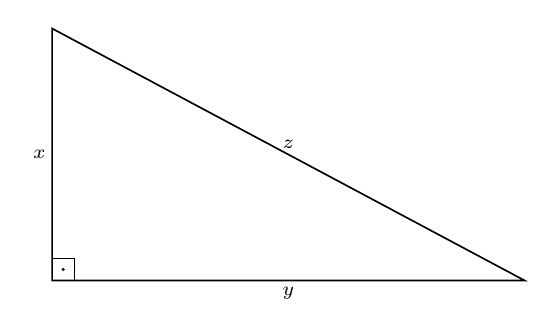
\begin{tikzpicture}[x=1.000cm,y=1.000cm,line width=0.6pt,baseline=(current bounding box.north)]\draw (0.000,0.000) -- (6.000,0.000) -- (0.000,3.200) -- cycle;\draw[line width=0.4pt] (0.280,0.000) -- (0.280,0.280) -- (0.000,0.280);\fill (0.140,0.140) circle (0.6pt);\node[font=\scriptsize,anchor=east,inner sep=2pt] at (0.000,1.600) {$x$};\node[font=\scriptsize,anchor=north,inner sep=2pt] at (3.000,0.000) {$y$};\node[font=\scriptsize,anchor=south,inner sep=2pt] at (3.000,1.600) {$z$};\end{tikzpicture}\par
\fusshilfe{\mbox{13:~z² = x² + y²}}
\end{pfaufg}
\begin{pfaufg}{P10 ’21}{14.}{}
Im abgebildeten Dreieck sind x und y die Katheten, z ist die Hypotenuse. Kreuze die Formel an, mit der man z berechnet:
\pfkreuzzeile{$z=\sqrt{x^2-y^2}$}\pfkreuzzeile{$z=\sqrt{x^2+y^2}$}\pfkreuzzeile{$z=\sqrt{y^2-x^2}$}\pfkreuzzeile{$z=y^2+x^2$}
\par\smallskip\noindent 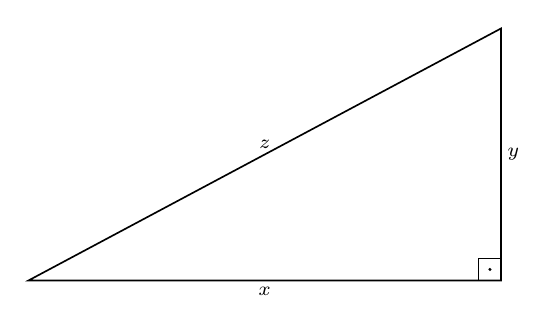
\begin{tikzpicture}[x=1.000cm,y=1.000cm,line width=0.6pt,baseline=(current bounding box.north)]\draw (6.000,0.000) -- (0.000,0.000) -- (6.000,3.200) -- cycle;\draw[line width=0.4pt] (6.000,0.280) -- (5.720,0.280) -- (5.720,0.000);\fill (5.860,0.140) circle (0.6pt);\node[font=\scriptsize,anchor=north,inner sep=2pt] at (3.000,0.000) {$x$};\node[font=\scriptsize,anchor=west,inner sep=2pt] at (6.000,1.600) {$y$};\node[font=\scriptsize,anchor=south,inner sep=2pt] at (3.000,1.600) {$z$};\end{tikzpicture}\par
\fusshilfe{\mbox{14:~z = √(x² + y²)}}
\end{pfaufg}
\begin{pfaufg}{P10 ’24}{15.}{}
Im abgebildeten Dreieck sind y und z die Katheten, x ist die Hypotenuse. Kreuze die Gleichung an, mit der man die Länge von z berechnen kann:
\pfkreuzzeile{$z=x^2-y^2$}\pfkreuzzeile{$z=\sqrt{x^2+y^2}$}\pfkreuzzeile{$z=x+y$}\pfkreuzzeile{$z=\sqrt{x^2-y^2}$}
\par\smallskip\noindent 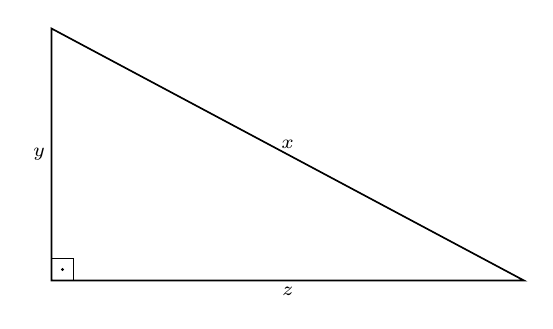
\begin{tikzpicture}[x=1.000cm,y=1.000cm,line width=0.6pt,baseline=(current bounding box.north)]\draw (0.000,0.000) -- (6.000,0.000) -- (0.000,3.200) -- cycle;\draw[line width=0.4pt] (0.280,0.000) -- (0.280,0.280) -- (0.000,0.280);\fill (0.140,0.140) circle (0.6pt);\node[font=\scriptsize,anchor=east,inner sep=2pt] at (0.000,1.600) {$y$};\node[font=\scriptsize,anchor=north,inner sep=2pt] at (3.000,0.000) {$z$};\node[font=\scriptsize,anchor=south,inner sep=2pt] at (3.000,1.600) {$x$};\end{tikzpicture}\par
\fusshilfe{\mbox{15:~z = √(x² $-$ y²) (vierte Option)}}
\end{pfaufg}
\pfgruppe{}
\begin{pfaufg}{P10 ’26}{16.}{}
Im abgebildeten Dreieck sind u und v die Katheten, w ist die Hypotenuse. Kreuze an, mit welcher Gleichung man w berechnen kann:
\pfkreuzzeile{$w=\sqrt{v^2-u^2}$}\pfkreuzzeile{$w=\sqrt{u^2-v^2}$}\pfkreuzzeile{$w=\sqrt{u^2+v^2}$}
\par\smallskip\noindent 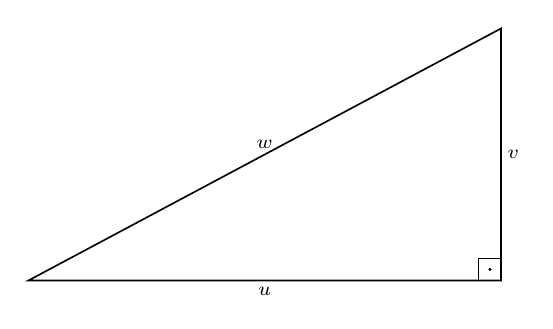
\begin{tikzpicture}[x=1.000cm,y=1.000cm,line width=0.6pt,baseline=(current bounding box.north)]\draw (6.000,0.000) -- (0.000,0.000) -- (6.000,3.200) -- cycle;\draw[line width=0.4pt] (6.000,0.280) -- (5.720,0.280) -- (5.720,0.000);\fill (5.860,0.140) circle (0.6pt);\node[font=\scriptsize,anchor=north,inner sep=2pt] at (3.000,0.000) {$u$};\node[font=\scriptsize,anchor=west,inner sep=2pt] at (6.000,1.600) {$v$};\node[font=\scriptsize,anchor=south,inner sep=2pt] at (3.000,1.600) {$w$};\end{tikzpicture}\par
\fusshilfe{\mbox{16:~w = √(u² + v²) (dritte Option)}}
\end{pfaufg}
\pfstufekopf[skatheteoderhypotenus]{Kathete oder Hypotenuse direkt}{in 3 der letzten 5 Prüfungen}
\pfgruppe{}
\begin{pfaufg}{}{17.}{}
Ein rechtwinkliges Dreieck hat diese drei Seiten. Kreuze an, welche Seite die Hypotenuse sein kann. 
\pfkreuzzeile{$4$ cm}\pfkreuzzeile{$8{,}5$ cm}\pfkreuzzeile{$7{,}5$ cm}
\fusshilfe{\mbox{17:~$8{,}5$ cm}}
\end{pfaufg}
\begin{pfaufg}{}{18.}{}
Die Figur zeigt ein gleichschenkliges Trapez mit seiner Höhe. Fahre das rechtwinklige Dreieck aus Höhe, Schenkel und Überstand farbig nach. Schreibe dazu, welche Seiten Katheten sind und welche die Hypotenuse ist.
\par\smallskip\noindent \trapez[hoehe=h]{5}{3}{2.5}\par
\rechenplatz{1}
\fusshilfe{\mbox{18:~Katheten: die Höhe und der Überstand}}
\end{pfaufg}
\pfgruppe{}
\begin{pfaufg}{P10 ’20}{19.}{}
Im Dreieck ABC ist bei C ein rechter Winkel. Die Strecke BC ist 12 m lang, die Strecke AC 34 m. Berechne die Länge der Strecke AB.
\par\smallskip\noindent \begin{tikzpicture}[x=1.000cm,y=1.000cm,line width=0.6pt,baseline=(current bounding box.north)]\draw (0.000,3.500) -- (6.000,3.500) -- (0.000,0.000) -- cycle;\draw[dashed] (0.000,2.800) -- (6.000,3.500);\draw[line width=0.4pt] (0.000,3.220) -- (0.280,3.220) -- (0.280,3.500);\fill (0.140,3.360) circle (0.6pt);\node[font=\small,inner sep=1pt] at (-0.259,3.651) {$C$};\node[font=\small,inner sep=1pt] at (6.288,3.584) {$B$};\node[font=\small,inner sep=1pt] at (-0.195,-0.228) {$A$};\node[font=\small,inner sep=1pt] at (-0.292,2.868) {$Q$};\fill (0.000,2.800) circle (1.4pt);\node[font=\scriptsize,mbgrau,anchor=north west] at ([yshift=-2pt]current bounding box.south west) {nicht maßstabsgerecht};\end{tikzpicture}\par
\rechenplatz{2}
\fusshilfe{\mbox{19:~AB = 10√13 $\approx$ 36,1 m}}
\end{pfaufg}
\begin{pfaufg}{P10 ’16}{20.}{}
An einem Fluss liegen der Bioladen C, eine Brücke D und eine Anlegestelle B auf einer Geraden am Ufer, in dieser Reihenfolge. Von einem Ausflugslokal A führt ein 920 m langer Weg zum Bioladen; vom Bioladen bis zur Brücke sind es 541 m. Die Strecke AD steht senkrecht auf dem Ufer. Am Bioladen ist der Winkel zwischen den Wegen nach A und nach D 54° groß, am Lokal der Winkel zwischen den Richtungen nach C und nach B 70°. Vom Lokal A soll ein neuer Weg direkt zur Brücke D führen. Ermittle die Länge von AD.
\par\smallskip\noindent \begin{tikzpicture}[line width=0.6pt,baseline=(current bounding box.north)]\draw (-0.6,3.12) -- (6.4,1.72);\draw (2.49,-0.15) -- (0.00,3.00);\draw (2.49,-0.15) -- (5.60,1.88);\draw[dashed] (2.49,-0.15) -- (3.00,2.40);\node[font=\small,anchor=south] at (0.00,3.00) {$C$};\node[font=\small,anchor=south] at (3.00,2.40) {$D$};\node[font=\small,anchor=south] at (5.60,1.88) {$B$};\node[font=\small,anchor=north] at (2.49,-0.15) {$A$};\path (2.49,-0.15) -- node[font=\scriptsize,left] {920 m} (0.00,3.00);\path (0.00,3.00) -- node[font=\scriptsize,above] {541 m} (3.00,2.40);\draw[line width=0.4pt] (0.00,3.00) ++(308.33096706931855:0.55) arc (308.33096706931855:348.69006752597977:0.55);\node[font=\scriptsize,fill=white,inner sep=0.5pt] at ($(0.00,3.00)+(328.51051729764913:0.8500000000000001)$) {54°};\draw[line width=0.4pt] (2.49,-0.15) ++(33.128308197129584:0.7) arc (33.128308197129584:128.33096706931855:0.7);\node[font=\scriptsize,fill=white,inner sep=0.5pt] at ($(2.49,-0.15)+(80.72963763322406:1.0)$) {70°};\draw[line width=0.4pt] (2.95,2.15) -- (3.20,2.11) -- (3.25,2.35);\node[font=\scriptsize,mbgrau,anchor=west] at (6.4,1.72) {Ufer};\node[font=\scriptsize,mbgrau,anchor=north west] at ([yshift=-2pt]current bounding box.south west) {nicht maßstabsgerecht};\end{tikzpicture}\par
\rechenplatz{2}
\fusshilfe{\mbox{20:~AD = √553 719 $\approx$ 744 m}}
\end{pfaufg}
\begin{pfaufg}{P10 ’19}{21.}{}
Beim Fußballtraining spielen sich drei Kinder den Ball zu: Amir steht bei A, Ben bei B, Chris bei C. Zwischen Ben und Amir sind es 4 m, zwischen Amir und Chris 9 m. Bei B ist ein rechter Winkel; der Winkel bei A heißt $\alpha$. Ermittle den Abstand zwischen Ben und Chris.
\par\smallskip\noindent \begin{tikzpicture}[x=1.000cm,y=1.000cm,line width=0.6pt,baseline=(current bounding box.north)]\draw (0.000,0.000) -- (0.000,3.500) -- (6.000,0.000) -- cycle;\draw[line width=0.4pt] (0.280,0.000) -- (0.280,0.280) -- (0.000,0.280);\fill (0.140,0.140) circle (0.6pt);\draw[line width=0.4pt] (0.000,3.080) arc (-90.00:-30.26:0.420);\node[font=\scriptsize,inner sep=0.5pt,fill=white] at (0.369,2.858) {$\alpha$};\node[font=\scriptsize,anchor=east,inner sep=2pt] at (0.000,1.750) {4 m};\node[font=\scriptsize,anchor=south,inner sep=2pt] at (3.000,1.750) {9 m};\node[font=\small,inner sep=1pt] at (-0.259,-0.151) {$B$};\node[font=\small,inner sep=1pt] at (-0.195,3.728) {$A$};\node[font=\small,inner sep=1pt] at (6.288,-0.084) {$C$};\node[font=\scriptsize,mbgrau,anchor=north west] at ([yshift=-2pt]current bounding box.south west) {nicht maßstabsgerecht};\end{tikzpicture}\par
\rechenplatz{2}
\fusshilfe{\mbox{21:~BC = √65 $\approx$ 8,06 m}}
\end{pfaufg}
\pfgruppe{}
\begin{pfaufg}{P10 ’22}{22.}{}
Gegeben ist ein Dreieck ABC, das nicht rechtwinklig ist. Die Höhe $h_c$ von C auf die Seite AB ist etwa 7,4 m lang; ihr Fußpunkt heißt D. Die Seite b = AC ist 14,1 m lang, der Winkel bei B ist 52° groß. Der Winkel bei C zwischen AC und der Höhe heißt $\gamma_1$. Weise nach, dass die Strecke AD etwa 12,0 m lang ist.
\par\smallskip\noindent \begin{tikzpicture}[x=1.000cm,y=1.000cm,line width=0.6pt,baseline=(current bounding box.north)]\draw (0.000,0.000) -- (6.000,0.000) -- (3.000,3.500) -- cycle;\draw[dashed] (3.000,3.500) -- (3.000,0.000);\draw[line width=0.4pt] (3.000,0.280) -- (2.720,0.280) -- (2.720,0.000);\fill (2.860,0.140) circle (0.6pt);\draw[line width=0.4pt] (0.420,0.000) arc (0.00:49.40:0.420);\node[font=\scriptsize,inner sep=0.5pt,fill=white] at (0.672,0.309) {$\alpha$};\draw[line width=0.4pt] (5.727,0.319) arc (130.60:180.00:0.420);\node[font=\scriptsize,inner sep=0.5pt,fill=white] at (5.164,0.384) {52°};\draw[line width=0.4pt] (3.000,3.080) arc (-90.00:0.00:0.420);\node[font=\scriptsize,inner sep=0.5pt,fill=white] at (3.523,2.977) {$\gamma_1$};\node[font=\scriptsize,anchor=west,inner sep=2pt] at (3.000,1.750) {$h_c$};\node[font=\scriptsize,anchor=east,inner sep=2pt] at (1.500,1.750) {b = 14,1 m};\node[font=\scriptsize,anchor=west,inner sep=2pt] at (4.500,1.750) {a};\node[font=\small,inner sep=1pt] at (-0.280,-0.109) {$A$};\node[font=\small,inner sep=1pt] at (6.280,-0.109) {$B$};\node[font=\small,inner sep=1pt] at (3.000,3.800) {$C$};\node[font=\small,inner sep=1pt] at (3.000,-0.300) {$D$};\node[font=\scriptsize,mbgrau,anchor=north west] at ([yshift=-2pt]current bounding box.south west) {nicht maßstabsgerecht};\end{tikzpicture}\par
\rechenplatz{2}
\fusshilfe{\mbox{22:~AD = √(14,1² $-$ 7,4²) $\approx$ 12,0 m}}
\end{pfaufg}
\pfgruppe{}
\begin{pfaufg}{P10 ’24}{23.}{}
Eine Seilbahn führt vom Ort B im Tal zum Ort A auf einem Berg. F liegt senkrecht unter A auf der Höhe von B; bei F ist ein rechter Winkel. FB ist 255 m lang, die Seilbahnstrecke AB 384 m. Eine zweite Seilbahn verbindet B mit dem Ort C auf einem anderen Berg. Bei B heißt der Winkel zwischen BF und BA $\beta_1$, der Winkel zwischen BA und BC $\beta_2$; bei A heißt der Winkel zwischen AB und AC $\alpha$. Die Strecke FA ist der Höhenunterschied zwischen B und A. Berechne diesen Höhenunterschied.
\par\smallskip\noindent \begin{tikzpicture}[x=1.000cm,y=1.000cm,line width=0.6pt,baseline=(current bounding box.north)]\draw (0.000,3.500) -- (0.000,0.000) -- (6.000,0.000) -- cycle;\draw[] (6.000,3.500) -- (0.000,3.500);\draw[] (6.000,3.500) -- (6.000,0.000);\draw[line width=0.4pt] (0.280,0.000) -- (0.280,0.280) -- (0.000,0.280);\fill (0.140,0.140) circle (0.6pt);\draw[line width=0.4pt] (5.352,0.378) arc (149.74:180.00:0.750);\node[font=\scriptsize,inner sep=0.5pt,fill=white] at (4.967,0.279) {$\beta_1$};\draw[line width=0.4pt] (6.000,0.420) arc (90.00:149.74:0.420);\node[font=\scriptsize,inner sep=0.5pt,fill=white] at (5.631,0.642) {$\beta_2$};\draw[line width=0.4pt] (0.000,3.080) arc (-90.00:-30.26:0.420);\node[font=\scriptsize,inner sep=0.5pt,fill=white] at (0.369,2.858) {$\alpha$};\node[font=\scriptsize,anchor=north,inner sep=2pt] at (3.000,0.000) {255 m};\node[font=\scriptsize,anchor=south,inner sep=2pt] at (3.000,1.750) {384 m};\node[font=\small,inner sep=1pt] at (-0.195,3.728) {$A$};\node[font=\small,inner sep=1pt] at (6.259,3.651) {$C$};\node[font=\small,inner sep=1pt] at (-0.259,-0.151) {$F$};\node[font=\small,inner sep=1pt] at (6.288,-0.084) {$B$};\node[font=\scriptsize,mbgrau,anchor=north west] at ([yshift=-2pt]current bounding box.south west) {nicht maßstabsgerecht};\end{tikzpicture}\par
\rechenplatz{2}
\fusshilfe{\mbox{23:~FA = 3√9159 $\approx$ 287,1 m}}
\end{pfaufg}
\pfgruppe{}
\begin{pfaufg}{P10 ’22}{\llap{\textasteriskcentered\,}24.}{}
Ein Becher hat die Form eines Zylinders ohne Deckel. Er ist h = 7 cm hoch und hat den Radius r = 3,2 cm. Ein Becher hat die Form eines Zylinders ohne Deckel; er ist 7 cm hoch und hat den Radius 3,2 cm. Ein Rührstab steht schräg im Becher: Er berührt unten den Rand des Bodens und lehnt oben am gegenüberliegenden Rand. 2 cm des Stabs ragen über den Becher hinaus. Bestimme die Länge des Stabs.
\par\smallskip\noindent \begin{tikzpicture}[line width=0.6pt,baseline=(current bounding box.north)]\draw (-1.10,0.00) arc (180:360:1.10 and 0.33);\draw[dashed] (1.10,0.00) arc (0:180:1.10 and 0.33);\draw (-1.1,0) -- (-1.1,2.4); \draw (1.1,0) -- (1.1,2.4);\draw (0,2.4) ellipse (1.1 and 0.33);\draw[line width=1.6pt] (-0.99,-0.15) -- (1.38,3.15);\node[font=\scriptsize,mbgrau,anchor=north west] at ([yshift=-2pt]current bounding box.south west) {nicht maßstabsgerecht};\end{tikzpicture}\par
\rechenplatz{3}
\fusshilfe{\mbox{24:~√89,96 + 2 $\approx$ 11,5 cm}}
\end{pfaufg}

\pfstufekopf[sdreieckerstinfigurod]{Dreieck erst in Figur oder Körper finden}{in 2 der letzten 5 Prüfungen}
\pfgruppe{}
\begin{pfaufg}{}{25.}{}
Die Figur zeigt einen Kegel. Sein Durchmesser ist $18$ cm lang. Höhe, Radius und Mantellinie bilden ein rechtwinkliges Dreieck. Kreuze an, welche Länge in dieses Dreieck gehört. 
\pfkreuzzeile{$18$ cm}\pfkreuzzeile{$9$ cm}
\par\smallskip\noindent \kegel{1.5}{3}{}{}{}\par
\fusshilfe{\mbox{25:~$9$ cm}}
\end{pfaufg}
\begin{pfaufg}{}{26.}{}
Gilt für das Dreieck in der Figur der Satz des Pythagoras? \janein
\par\smallskip\noindent \dreieckrw{5}{3.57}{}{}{}\par
\fusshilfe{\mbox{26:~rechter Winkel bei C}}
\end{pfaufg}
\pfgruppe{}
\begin{pfaufg}{P10 ’18}{\llap{\textasteriskcentered\,}27.}{}
Ein runder Turm mit 6,4 m Durchmesser hat ein Dach in Form eines Kegels. Die Höhe des Daches ist bekannt. Ein Dachbalken läuft von der Spitze bis zum Rand des Daches. Beschreibe, wie man die Länge eines Dachbalkens berechnen kann.
\par\smallskip\noindent \begin{tikzpicture}[line width=0.6pt,baseline=(current bounding box.north)]\draw (-1.20,0.00) arc (180:360:1.20 and 0.36);\draw[dashed] (1.20,0.00) arc (0:180:1.20 and 0.36);\draw (-1.2,0) -- (0,2.4) -- (1.2,0);\draw[-{Stealth[length=2mm]},line width=0.4pt] (1.9,1.9) node[right,font=\scriptsize] {Dachbalken} -- (0.5,1.4);\node[font=\scriptsize,mbgrau,anchor=north west] at ([yshift=-2pt]current bounding box.south west) {nicht maßstabsgerecht};\end{tikzpicture}\par
\rechenplatz{2}
\fusshilfe{\mbox{27:~s = √(3,2² + h²)}}
\end{pfaufg}
\pfgruppe{}
\begin{pfaufg}{P10 ’26}{\llap{\textasteriskcentered\,}28.}{}
Ein Turm besteht unten aus einem Zylinder, sein Dach ist ein Kegel. Bekannt sind: h = 25,0 m (Höhe des Zylinders), r = 4,7 m (Radius von Zylinder und Kegel) und s = 8,6 m (Mantellinie des Kegels). Ein Turm besteht aus einem Zylinder (Höhe 25,0 m, Radius 4,7 m) mit einem Kegeldach; die Mantellinie des Kegels ist 8,6 m lang, sein Radius ebenfalls 4,7 m. Bestimme die Gesamthöhe des Turms.
\par\smallskip\noindent \begin{tikzpicture}[line width=0.6pt,baseline=(current bounding box.north)]\draw (-1.00,0.00) arc (180:360:1.00 and 0.30);\draw[dashed] (1.00,0.00) arc (0:180:1.00 and 0.30);\draw (-1.0,0) -- (-1.0,2.6); \draw (1.0,0) -- (1.0,2.6);\draw (-1.00,2.60) arc (180:360:1.00 and 0.30);\draw[dashed] (1.00,2.60) arc (0:180:1.00 and 0.30);\draw (-1.0,2.6) -- (0,3.9000000000000004) -- (1.0,2.6);\draw[dashed] (0,2.6) -- (1.0,2.6);\node[font=\scriptsize,right] at (1.0,1.3) {$h$ = 25,0 m};\node[font=\scriptsize,below,fill=white,inner sep=1pt] at (0.5,2.52) {$r$ = 4,7 m};\node[font=\scriptsize,right] at (0.55,3.35) {$s$ = 8,6 m};\node[font=\scriptsize,mbgrau,anchor=north west] at ([yshift=-2pt]current bounding box.south west) {nicht maßstabsgerecht};\end{tikzpicture}\par
\rechenplatz{3}
\fusshilfe{\mbox{28:~25 + √51,87 $\approx$ 32,2 m}}
\end{pfaufg}
\begin{pfaufg}{P10 ’25}{29.}{}
Familie Yücel baut an die Stufe vor der Haustür eine feste Rampe für Rollstühle. Die Stufe ist 16 cm hoch; waagerecht ist die Rampe 170 cm lang. Berechne die Länge x der Rampe. Berechne den Anstiegswinkel $\alpha$.
\par\smallskip\noindent \begin{tikzpicture}[line width=0.6pt]\draw (0,0) -- (6,0) -- (6,1.4) -- cycle;\draw (5.7,0) -- (5.7,0.3) -- (6,0.3);\node[below,font=\small] at (3,0) {170 cm};\node[right,font=\small] at (6,0.7) {16 cm};\node[above left,font=\small] at (3,0.7) {$x$};\node[font=\small] at (1.1,0.12) {$\alpha$};\node[font=\scriptsize,mbgrau,anchor=west] at (0,-0.75) {nicht maßstabsgerecht};\end{tikzpicture}\par
\rechenplatz{3}
\fusshilfe{\mbox{29:~x = 2√7289 $\approx$ 170,8 cm; $\alpha$ = tan$^{-1}$($\tfrac{8}{85}$) $\approx$ 5,4°}}
\end{pfaufg}
\pfgruppe{}
\begin{pfaufg}{P10 ’19}{30.}{}
Im Koordinatensystem bilden die Punkte A(0|$-$2), B(2|$-$2) und C(0|2) ein Dreieck. Berechne die Länge der Strecke BC. Berechne die Größe des Winkels $\beta$ bei B.
\par\smallskip\noindent \begin{tikzpicture}\begin{axis}[xmin=-5,xmax=5,ymin=-5,ymax=5,axis lines=middle,tick label style={font=\scriptsize},clip=true,/pgf/number format/use comma,axis line style={-{Stealth[length=2mm]}},every axis plot/.append style={line width=0.9pt},x=0.9cm,y=0.9cm,xtick distance=1,ytick distance=1,enlargelimits=false,grid=both,grid style={mbgitter,line width=0.3pt},major grid style={mbgitter},minor tick num=1,xlabel={$x$},ylabel={$y$},x label style={anchor=west},y label style={anchor=south}]\draw[line width=0.8pt] (axis cs:0,-2) -- (axis cs:2,-2) -- (axis cs:0,2) -- cycle;\fill (axis cs:0,-2) circle (1.6pt) node[above right,font=\small,inner sep=1pt] {$A$};\fill (axis cs:2,-2) circle (1.6pt) node[above right,font=\small,inner sep=1pt] {$B$};\fill (axis cs:0,2) circle (1.6pt) node[above right,font=\small,inner sep=1pt] {$C$};\draw[line width=0.5pt] (axis cs:2,-2) ++(116.5651:0.55cm) arc (116.5651:180:0.55cm);\node[font=\small] at ($(axis cs:2,-2)+(148.2825:0.85cm)$) {$\beta$};\end{axis}\end{tikzpicture}\par
\rechenplatz{4}
\fusshilfe{\mbox{30:~BC = √20 $\approx$ 4,47; $\beta$ = tan$^{-1}$(2) $\approx$ 63,4°}}
\end{pfaufg}
\pfsteckt{steckt auch in Nr. 94 (P10 ’25)}
\pfstufekopf[sseitenverhltnisbenen]{Seitenverhältnis benennen}{in 1 der letzten 5 Prüfungen}
\pfgruppe{}
\begin{pfaufg}{}{31.}{}
Mit der Gleichung $\mathrm{sin}\,23^\circ = \tfrac{x}{8}$ soll die Seite $x$ berechnet werden. Kreuze an, ob du dafür mal nimmst oder teilst. 
\pfkreuzzeile{im Zähler: mal}\pfkreuzzeile{im Nenner: geteilt}
\fusshilfe{\mbox{31:~im Zähler: mal}}
\end{pfaufg}
\begin{pfaufg}{}{32.}{}
Die Figur zeigt ein Dreieck mit rechtem Winkel bei $B$. Schau vom Winkel $\alpha$ aus. Schreibe an jede Seite H (Hypotenuse), G (Gegenkathete) oder A (Ankathete).
\par\smallskip\noindent \dreieck{(0,0)}{(5,0)}{(5,3)}{r}{t}{s}{\alpha}{}{}\par
\rechenplatz{1}
\fusshilfe{\mbox{32:~r: G, s: A, t: H}}
\end{pfaufg}
\pfgruppe{}
\begin{pfaufg}{P10 ’20}{33.}{}
Für x gilt die Gleichung $\sin 30^\circ=\tfrac{7}{x}$. Gib den Wert von x an.
\rechenplatz{2}
\fusshilfe{\mbox{33:~x = 14}}
\end{pfaufg}
\pfgruppe{}
\begin{pfaufg}{P10 ’17}{34.}{}
Schreibe $\sin\beta$ als Verhältnis zweier Seiten des abgebildeten Dreiecks.
\par\smallskip\noindent 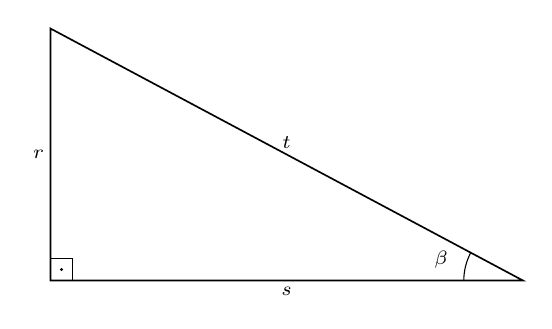
\begin{tikzpicture}[x=1.000cm,y=1.000cm,line width=0.6pt,baseline=(current bounding box.north)]\draw (0.000,0.000) -- (6.000,0.000) -- (0.000,3.200) -- cycle;\draw[line width=0.4pt] (0.280,0.000) -- (0.280,0.280) -- (0.000,0.280);\fill (0.140,0.140) circle (0.6pt);\draw[line width=0.4pt] (5.338,0.353) arc (151.93:180.00:0.750);\node[font=\scriptsize,inner sep=0.5pt,fill=white] at (4.962,0.260) {$\beta$};\node[font=\scriptsize,anchor=east,inner sep=2pt] at (0.000,1.600) {$r$};\node[font=\scriptsize,anchor=north,inner sep=2pt] at (3.000,0.000) {$s$};\node[font=\scriptsize,anchor=south,inner sep=2pt] at (3.000,1.600) {$t$};\end{tikzpicture}\par
\rechenplatz{1}
\fusshilfe{\mbox{34:~sin $\beta$ = r/t}}
\end{pfaufg}
\begin{pfaufg}{P10 ’19}{35.}{}
Schreibe $\sin\alpha$ als Verhältnis zweier Seiten des abgebildeten Dreiecks.
\par\smallskip\noindent 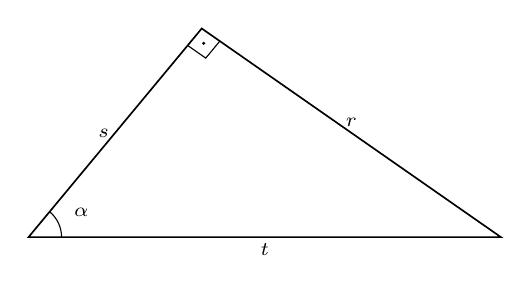
\begin{tikzpicture}[x=1.000cm,y=1.000cm,line width=0.6pt,baseline=(current bounding box.north)]\draw (0.000,0.000) -- (6.000,0.000) -- (2.200,2.650) -- cycle;\draw[line width=0.4pt] (2.021,2.435) -- (2.251,2.274) -- (2.430,2.490);\fill (2.225,2.462) circle (0.6pt);\draw[line width=0.4pt] (0.420,0.000) arc (0.00:50.30:0.420);\node[font=\scriptsize,inner sep=0.5pt,fill=white] at (0.670,0.314) {$\alpha$};\node[font=\scriptsize,anchor=north,inner sep=2pt] at (3.000,0.000) {$t$};\node[font=\scriptsize,anchor=east,inner sep=2pt] at (1.100,1.325) {$s$};\node[font=\scriptsize,anchor=south,inner sep=2pt] at (4.100,1.325) {$r$};\end{tikzpicture}\par
\rechenplatz{1}
\fusshilfe{\mbox{35:~sin $\alpha$ = r/t}}
\end{pfaufg}
\begin{pfaufg}{P10 ’20}{36.}{}
Schreibe $\tan\alpha$ als Verhältnis zweier Seiten des abgebildeten Dreiecks.
\par\smallskip\noindent 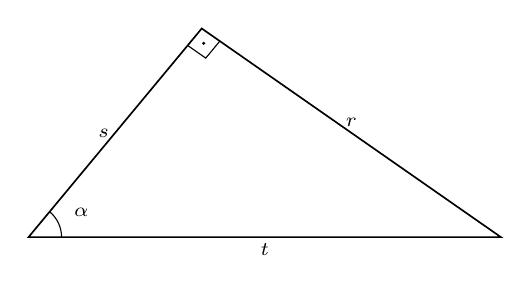
\begin{tikzpicture}[x=1.000cm,y=1.000cm,line width=0.6pt,baseline=(current bounding box.north)]\draw (0.000,0.000) -- (6.000,0.000) -- (2.200,2.650) -- cycle;\draw[line width=0.4pt] (2.021,2.435) -- (2.251,2.274) -- (2.430,2.490);\fill (2.225,2.462) circle (0.6pt);\draw[line width=0.4pt] (0.420,0.000) arc (0.00:50.30:0.420);\node[font=\scriptsize,inner sep=0.5pt,fill=white] at (0.670,0.314) {$\alpha$};\node[font=\scriptsize,anchor=east,inner sep=2pt] at (1.100,1.325) {$s$};\node[font=\scriptsize,anchor=south,inner sep=2pt] at (4.100,1.325) {$r$};\node[font=\scriptsize,anchor=north,inner sep=2pt] at (3.000,0.000) {$t$};\end{tikzpicture}\par
\rechenplatz{1}
\fusshilfe{\mbox{36:~tan $\alpha$ = r/s}}
\end{pfaufg}
\begin{pfaufg}{P10 ’25}{37.}{}
Ergänze die Gleichung passend zur Abbildung: $\sin\gamma=$ \_\_\_
\par\smallskip\noindent 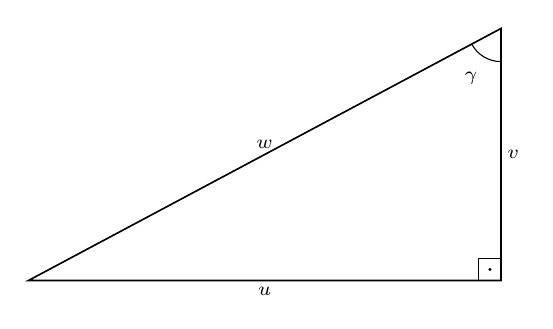
\begin{tikzpicture}[x=1.000cm,y=1.000cm,line width=0.6pt,baseline=(current bounding box.north)]\draw (6.000,0.000) -- (0.000,0.000) -- (6.000,3.200) -- cycle;\draw[line width=0.4pt] (6.000,0.280) -- (5.720,0.280) -- (5.720,0.000);\fill (5.860,0.140) circle (0.6pt);\draw[line width=0.4pt] (5.629,3.002) arc (-151.93:-90.00:0.420);\node[font=\scriptsize,inner sep=0.5pt,fill=white] at (5.619,2.565) {$\gamma$};\node[font=\scriptsize,anchor=north,inner sep=2pt] at (3.000,0.000) {$u$};\node[font=\scriptsize,anchor=west,inner sep=2pt] at (6.000,1.600) {$v$};\node[font=\scriptsize,anchor=south,inner sep=2pt] at (3.000,1.600) {$w$};\end{tikzpicture}\par
\rechenplatz{1}
\fusshilfe{\mbox{37:~sin $\gamma$ = u/w}}
\end{pfaufg}
\pfgruppe{}
\begin{pfaufg}{P10 ’18}{38.}{}
Im abgebildeten Dreieck ist a die Hypotenuse, b die Kathete gegenüber von $\beta$. Kreuze die Gleichung an, mit der man $\beta$ berechnen kann:
\pfkreuzzeile{$\sin\beta=\tfrac{a}{b}$}\pfkreuzzeile{$\cos\beta=\tfrac{a}{b}$}\pfkreuzzeile{$\sin\beta=\tfrac{b}{a}$}
\par\smallskip\noindent 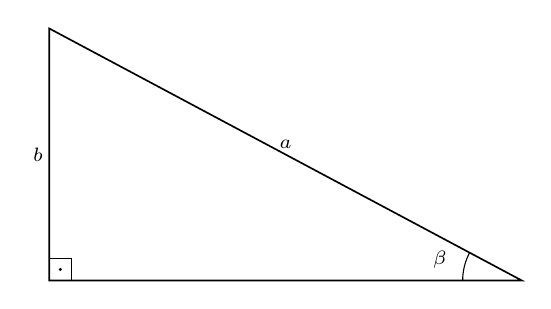
\begin{tikzpicture}[x=1.000cm,y=1.000cm,line width=0.6pt,baseline=(current bounding box.north)]\draw (0.000,0.000) -- (6.000,0.000) -- (0.000,3.200) -- cycle;\draw[line width=0.4pt] (0.280,0.000) -- (0.280,0.280) -- (0.000,0.280);\fill (0.140,0.140) circle (0.6pt);\draw[line width=0.4pt] (5.338,0.353) arc (151.93:180.00:0.750);\node[font=\scriptsize,inner sep=0.5pt,fill=white] at (4.962,0.260) {$\beta$};\node[font=\scriptsize,anchor=east,inner sep=2pt] at (0.000,1.600) {$b$};\node[font=\scriptsize,anchor=south,inner sep=2pt] at (3.000,1.600) {$a$};\end{tikzpicture}\par
\fusshilfe{\mbox{38:~sin $\beta$ = b/a}}
\end{pfaufg}
\pfstufekopf[swinkelberechnen]{Winkel berechnen}{in 4 der letzten 5 Prüfungen}
\pfgruppe{}
\begin{pfaufg}{}{39.}{}
Ein rechtwinkliges Dreieck hat die Hypotenuse $7$ cm und die Gegenkathete $4$ cm. Du sollst den Winkel $\alpha$ berechnen. Kreuze an, was gesucht ist und wie du vorgehst. 
\pfkreuzzeile{Seite: Gleichung umstellen}\pfkreuzzeile{Winkel: Umkehrtaste}
\fusshilfe{\mbox{39:~Winkel: Umkehrtaste}}
\end{pfaufg}
\begin{pfaufg}{}{40.}{}
Die Figur zeigt ein Dreieck mit rechtem Winkel bei $B$. Vom Winkel $\alpha$ aus gesehen ist die Seite $a$ gegeben. Die Seite $b$ ist gesucht. Kreuze an, welche Funktion $a$ und $b$ verbindet. 
\pfkreuzzeile{sin}\pfkreuzzeile{cos}\pfkreuzzeile{tan}
\par\smallskip\noindent \dreieck{(0,0)}{(5,0)}{(5,3)}{a}{?}{c}{\alpha}{}{}\par
\fusshilfe{\mbox{40:~sin}}
\end{pfaufg}
\pfgruppe{}
\begin{pfaufg}{P10 ’19}{41.}{}
Beim Fußballtraining spielen sich drei Kinder den Ball zu: Amir steht bei A, Ben bei B, Chris bei C. Zwischen Ben und Amir sind es 4 m, zwischen Amir und Chris 9 m. Bei B ist ein rechter Winkel; der Winkel bei A heißt $\alpha$. Zeige mit einer Rechnung, dass $\alpha$ etwa 64° groß ist.
\par\smallskip\noindent \begin{tikzpicture}[x=1.000cm,y=1.000cm,line width=0.6pt,baseline=(current bounding box.north)]\draw (0.000,0.000) -- (0.000,3.500) -- (6.000,0.000) -- cycle;\draw[line width=0.4pt] (0.280,0.000) -- (0.280,0.280) -- (0.000,0.280);\fill (0.140,0.140) circle (0.6pt);\draw[line width=0.4pt] (0.000,3.080) arc (-90.00:-30.26:0.420);\node[font=\scriptsize,inner sep=0.5pt,fill=white] at (0.369,2.858) {$\alpha$};\node[font=\scriptsize,anchor=east,inner sep=2pt] at (0.000,1.750) {4 m};\node[font=\scriptsize,anchor=south,inner sep=2pt] at (3.000,1.750) {9 m};\node[font=\small,inner sep=1pt] at (-0.259,-0.151) {$B$};\node[font=\small,inner sep=1pt] at (-0.195,3.728) {$A$};\node[font=\small,inner sep=1pt] at (6.288,-0.084) {$C$};\node[font=\scriptsize,mbgrau,anchor=north west] at ([yshift=-2pt]current bounding box.south west) {nicht maßstabsgerecht};\end{tikzpicture}\par
\rechenplatz{2}
\fusshilfe{\mbox{41:~cos $\alpha$ = $\tfrac{4}{9}$ $\Rightarrow$ $\alpha$ $\approx$ 63,6° $\approx$ 64°}}
\end{pfaufg}
\begin{pfaufg}{P10 ’22}{42.}{}
Gegeben ist ein Dreieck ABC, das nicht rechtwinklig ist. Die Höhe $h_c$ von C auf die Seite AB ist etwa 7,4 m lang; ihr Fußpunkt heißt D. Die Seite b = AC ist 14,1 m lang, der Winkel bei B ist 52° groß. Der Winkel bei C zwischen AC und der Höhe heißt $\gamma_1$. Berechne die Größe des Winkels $\alpha$.
\par\smallskip\noindent \begin{tikzpicture}[x=1.000cm,y=1.000cm,line width=0.6pt,baseline=(current bounding box.north)]\draw (0.000,0.000) -- (6.000,0.000) -- (3.000,3.500) -- cycle;\draw[dashed] (3.000,3.500) -- (3.000,0.000);\draw[line width=0.4pt] (3.000,0.280) -- (2.720,0.280) -- (2.720,0.000);\fill (2.860,0.140) circle (0.6pt);\draw[line width=0.4pt] (0.420,0.000) arc (0.00:49.40:0.420);\node[font=\scriptsize,inner sep=0.5pt,fill=white] at (0.672,0.309) {$\alpha$};\draw[line width=0.4pt] (5.727,0.319) arc (130.60:180.00:0.420);\node[font=\scriptsize,inner sep=0.5pt,fill=white] at (5.164,0.384) {52°};\draw[line width=0.4pt] (3.000,3.080) arc (-90.00:0.00:0.420);\node[font=\scriptsize,inner sep=0.5pt,fill=white] at (3.523,2.977) {$\gamma_1$};\node[font=\scriptsize,anchor=west,inner sep=2pt] at (3.000,1.750) {$h_c$};\node[font=\scriptsize,anchor=east,inner sep=2pt] at (1.500,1.750) {b = 14,1 m};\node[font=\scriptsize,anchor=west,inner sep=2pt] at (4.500,1.750) {a};\node[font=\small,inner sep=1pt] at (-0.280,-0.109) {$A$};\node[font=\small,inner sep=1pt] at (6.280,-0.109) {$B$};\node[font=\small,inner sep=1pt] at (3.000,3.800) {$C$};\node[font=\small,inner sep=1pt] at (3.000,-0.300) {$D$};\node[font=\scriptsize,mbgrau,anchor=north west] at ([yshift=-2pt]current bounding box.south west) {nicht maßstabsgerecht};\end{tikzpicture}\par
\rechenplatz{2}
\fusshilfe{\mbox{42:~$\alpha$ = sin$^{-1}$($\tfrac{74}{141}$) $\approx$ 31,7°}}
\end{pfaufg}
\begin{pfaufg}{P10 ’24}{43.}{}
Eine Seilbahn führt vom Ort B im Tal zum Ort A auf einem Berg. F liegt senkrecht unter A auf der Höhe von B; bei F ist ein rechter Winkel. FB ist 255 m lang, die Seilbahnstrecke AB 384 m. Eine zweite Seilbahn verbindet B mit dem Ort C auf einem anderen Berg. Bei B heißt der Winkel zwischen BF und BA $\beta_1$, der Winkel zwischen BA und BC $\beta_2$; bei A heißt der Winkel zwischen AB und AC $\alpha$. Bestimme den Winkel $\beta_1$, unter dem die Seilbahn von B nach A ansteigt.
\par\smallskip\noindent \begin{tikzpicture}[x=1.000cm,y=1.000cm,line width=0.6pt,baseline=(current bounding box.north)]\draw (0.000,3.500) -- (0.000,0.000) -- (6.000,0.000) -- cycle;\draw[] (6.000,3.500) -- (0.000,3.500);\draw[] (6.000,3.500) -- (6.000,0.000);\draw[line width=0.4pt] (0.280,0.000) -- (0.280,0.280) -- (0.000,0.280);\fill (0.140,0.140) circle (0.6pt);\draw[line width=0.4pt] (5.352,0.378) arc (149.74:180.00:0.750);\node[font=\scriptsize,inner sep=0.5pt,fill=white] at (4.967,0.279) {$\beta_1$};\draw[line width=0.4pt] (6.000,0.420) arc (90.00:149.74:0.420);\node[font=\scriptsize,inner sep=0.5pt,fill=white] at (5.631,0.642) {$\beta_2$};\draw[line width=0.4pt] (0.000,3.080) arc (-90.00:-30.26:0.420);\node[font=\scriptsize,inner sep=0.5pt,fill=white] at (0.369,2.858) {$\alpha$};\node[font=\scriptsize,anchor=north,inner sep=2pt] at (3.000,0.000) {255 m};\node[font=\scriptsize,anchor=south,inner sep=2pt] at (3.000,1.750) {384 m};\node[font=\small,inner sep=1pt] at (-0.195,3.728) {$A$};\node[font=\small,inner sep=1pt] at (6.259,3.651) {$C$};\node[font=\small,inner sep=1pt] at (-0.259,-0.151) {$F$};\node[font=\small,inner sep=1pt] at (6.288,-0.084) {$B$};\node[font=\scriptsize,mbgrau,anchor=north west] at ([yshift=-2pt]current bounding box.south west) {nicht maßstabsgerecht};\end{tikzpicture}\par
\rechenplatz{2}
\fusshilfe{\mbox{43:~$\beta$1 = cos$^{-1}$($\tfrac{85}{128}$) $\approx$ 48,4°}}
\end{pfaufg}
\pfgruppe{}
\begin{pfaufg}{P10 ’20}{44.}{}
Eine Schachtel hat als Seitenfläche ein Trapez mit zwei rechten Winkeln: Die Grundseite ist 14 cm lang, die linke Seite 6 cm und die rechte Seite 15 cm hoch; beide stehen senkrecht auf der Grundseite. Die obere Seite verläuft schräg. Berechne den Winkel $\alpha$ oben rechts zwischen der rechten Seite und der schrägen Seite.
\par\smallskip\noindent \begin{tikzpicture}[x=1.000cm,y=1.000cm,line width=0.6pt,baseline=(current bounding box.north)]\draw (0.000,0.000) -- (6.000,0.000) -- (6.000,3.600) -- (0.000,1.600) -- cycle;\draw[dashed] (0.000,1.600) -- (6.000,1.600);\draw[line width=0.4pt] (0.280,0.000) -- (0.280,0.280) -- (0.000,0.280);\fill (0.140,0.140) circle (0.6pt);\draw[line width=0.4pt] (6.000,0.280) -- (5.720,0.280) -- (5.720,0.000);\fill (5.860,0.140) circle (0.6pt);\draw[line width=0.4pt] (5.602,3.467) arc (-161.57:-90.00:0.420);\node[font=\scriptsize,inner sep=0.5pt,fill=white] at (5.567,3.000) {$\alpha$};\node[font=\scriptsize,anchor=north,inner sep=2pt] at (3.000,0.000) {14 cm};\node[font=\scriptsize,anchor=east,inner sep=2pt] at (0.000,0.800) {6 cm};\node[font=\scriptsize,anchor=west,inner sep=2pt] at (6.000,1.800) {15 cm};\node[font=\scriptsize,mbgrau,anchor=north west] at ([yshift=-2pt]current bounding box.south west) {nicht maßstabsgerecht};\end{tikzpicture}\par
\rechenplatz{3}
\fusshilfe{\mbox{44:~$\alpha$ = tan$^{-1}$($\tfrac{14}{9}$) $\approx$ 57,3°}}
\end{pfaufg}
\pfsteckt{steckt auch in Nr. 30 (P10 ’19); Nr. 29 (P10 ’25)}
\pfstufekopf[sseiteberechnen]{Seite berechnen}{in 3 der letzten 5 Prüfungen}
\pfgruppe{}
\begin{pfaufg}{}{45.}{}
Die Figur zeigt ein Parallelogramm mit einer Höhe. Die Höhe bildet ein rechtwinkliges Teildreieck. Fahre es mit dem Stift nach. Schreibe an seine Seiten H (Hypotenuse), G (Gegenkathete) oder A (Ankathete). Schau dabei vom Winkel $\alpha$ aus.
\par\smallskip\noindent \parallelogramm[seiten={a,b,a,b},hoehe,winkel={\alpha,\beta,,}]{4}{2.5}{60}\par
\rechenplatz{1}
\end{pfaufg}
\begin{pfaufg}{}{46.}{}
Die Figur zeigt das Dreieck $ABC$. Zeichne die Höhe von $C$ auf die Seite $c$ ein. Fahre das linke Teildreieck mit dem Stift nach. Schreibe an seine Seiten H (Hypotenuse), G (Gegenkathete) oder A (Ankathete). Schau dabei vom Winkel $\alpha$ aus.
\par\smallskip\noindent \dreieck{(0,0)}{(6,0)}{(2,3)}{a}{b}{c}{\alpha}{\beta}{\gamma}\par
\rechenplatz{1}
\end{pfaufg}
\pfgruppe{}
\begin{pfaufg}{P10 ’18}{47.}{}
Lea will die Höhe eines Berges bestimmen. Auf der Bergspitze C steht eine 12,0 m hohe Aussichtsplattform, ihre Spitze heißt D. Lea peilt von einem Punkt A aus, der 1,5 m über dem Boden liegt. Zur Bergspitze C misst sie gegenüber der Waagerechten 30°, zur Plattformspitze D 35°. B ist der Punkt senkrecht unter C auf der Höhe von A; bei B ist ein rechter Winkel. Der Winkel zwischen den beiden Peillinien heißt $\gamma$, der Winkel bei D im Dreieck ACD heißt $\delta$. Gegeben: AC = 112,8 m. Ermittle die Höhe des Berges über dem Boden. Gib an, wie hoch über dem Boden die Spitze D der Plattform liegt.
\par\smallskip\noindent \begin{tikzpicture}[line width=0.6pt,baseline=(current bounding box.north)]\draw[dashed] (-0.4,0) -- (6.2,0);\draw (0,0) -- (0.00,0.60);\draw (0.00,0.60) -- (5.50,0.60) -- (5.50,4.20);\draw (0.00,0.60) -- (5.50,3.10); \draw (0.00,0.60) -- (5.50,4.20);\draw[line width=1.2pt] (5.50,3.10) -- (5.50,4.20);\node[font=\small,anchor=east] at (0.00,0.60) {$A$};\node[font=\small,anchor=north west] at (5.50,0.60) {$B$};\node[font=\small,anchor=west] at (5.50,3.10) {$C$};\node[font=\small,anchor=south] at (5.50,4.20) {$D$};\path (0.00,0.00) -- node[font=\scriptsize,left] {1,5 m} (0.00,0.60);\path (5.50,3.10) -- node[font=\scriptsize,right] {12,0 m} (5.50,4.20);\draw[line width=0.4pt] (0.00,0.60) ++(0:1.6) arc (0:24.4:1.6);\node[font=\scriptsize,fill=white,inner sep=0.5pt] at ($(0.00,0.60)+(12.2:1.9000000000000001)$) {30°};\draw[line width=0.4pt] (0.00,0.60) ++(24.4:2.4) arc (24.4:33.2:2.4);\node[font=\scriptsize,fill=white,inner sep=0.5pt] at ($(0.00,0.60)+(28.8:2.6999999999999997)$) {$\gamma$};\draw[line width=0.4pt] (5.50,0.85) -- (5.25,0.85) -- (5.25,0.60);\draw[line width=0.4pt] (5.50,4.20) ++(213.2:0.6) arc (213.2:270:0.6);\node[font=\scriptsize,fill=white,inner sep=0.5pt] at ($(5.50,4.20)+(241.6:0.8999999999999999)$) {$\delta$};\draw[line width=0.4pt] (0.00,0.60) ++(0:3.4) arc (0:33.2:3.4);\node[font=\scriptsize,fill=white,inner sep=0.5pt] at ($(0.00,0.60)+(16.6:3.6999999999999997)$) {35°};\node[font=\scriptsize,mbgrau,anchor=north west] at ([yshift=-2pt]current bounding box.south west) {nicht maßstabsgerecht};\end{tikzpicture}\par
\rechenplatz{3}
\fusshilfe{\mbox{47:~57,9 m; 69,9 m}}
\end{pfaufg}
\pfgruppe{}
\begin{pfaufg}{P10 ’15}{\llap{\textasteriskcentered\,}48.}{}
Gegeben ist ein Drachenviereck ABCD. Die Diagonale AC ist senkrecht (A unten, C oben), die Diagonale BD waagerecht (D links, B rechts); beide schneiden sich in E im rechten Winkel. Die Seite AD ist 4,1 cm lang. Im Dreieck ABD ist der Winkel bei A 123° und der Winkel bei B 36° groß; der Winkel bei D heißt $\delta$. Berechne die Länge der Diagonale BD.
\par\smallskip\noindent \begin{tikzpicture}[x=0.750cm,y=0.750cm,line width=0.6pt,baseline=(current bounding box.north)]\draw (3.000,0.000) -- (6.000,1.750) -- (3.000,3.500) -- (-2.000,1.750) -- cycle;\draw[] (3.000,0.000) -- (3.000,1.750);\draw[] (3.000,1.750) -- (3.000,3.500);\draw[] (6.000,1.750) -- (3.000,1.750);\draw[] (3.000,1.750) -- (-2.000,1.750);\draw[line width=0.4pt] (3.000,1.377) -- (3.373,1.377) -- (3.373,1.750);\fill (3.187,1.563) circle (0.6pt);\draw[line width=0.4pt] (3.484,0.282) arc (30.26:160.71:0.560);\node[font=\scriptsize,inner sep=0.5pt,fill=white] at (2.883,1.221) {123°};\draw[line width=0.4pt] (5.000,1.750) arc (180.00:210.26:1.000);\node[font=\scriptsize,inner sep=0.5pt,fill=white] at (4.391,1.315) {36°};\draw[line width=0.4pt] (-1.056,1.420) arc (-19.29:0.00:1.000);\node[font=\scriptsize,inner sep=0.5pt,fill=white] at (-0.593,1.511) {$\delta$};\node[font=\scriptsize,anchor=north,inner sep=2pt] at (0.500,0.875) {4,1 cm};\node[font=\small,inner sep=1pt] at (3.110,3.885) {$C$};\node[font=\small,inner sep=1pt] at (3.110,-0.385) {$A$};\node[font=\small,inner sep=1pt] at (-2.400,1.750) {$D$};\node[font=\small,inner sep=1pt] at (6.400,1.750) {$B$};\node[font=\small,inner sep=1pt] at (3.400,1.750) {$E$};\node[font=\scriptsize,mbgrau,anchor=north west] at ([yshift=-2pt]current bounding box.south west) {nicht maßstabsgerecht};\end{tikzpicture}\par
\rechenplatz{2}
\fusshilfe{\mbox{48:~BD = 4,1 · sin 123° : sin 36° $\approx$ 5,85 cm}}
\end{pfaufg}
\begin{pfaufg}{P10 ’17}{49.}{}
Ein Dachboden hat als Querschnitt das Dreieck ABC. Die Dachschräge AC ist 4,50 m lang. Der Winkel bei A beträgt 62,8°, der Winkel bei B 34,9°; der Winkel bei C heißt $\gamma$. Auf dem Boden AB steht im Punkt P eine senkrechte Wand, die genau bis zur Dachschräge BC reicht. Sie ist 1,20 m hoch. Berechne den Abstand von P bis B.
\par\smallskip\noindent \begin{tikzpicture}[x=1.000cm,y=1.000cm,line width=0.6pt,baseline=(current bounding box.north)]\draw (0.000,0.000) -- (6.000,0.000) -- (2.000,3.500) -- cycle;\draw[line width=1.2pt] (4.800,0.000) -- (4.800,1.050);\draw[line width=0.4pt] (4.800,0.280) -- (4.520,0.280) -- (4.520,0.000);\fill (4.660,0.140) circle (0.6pt);\draw[line width=0.4pt] (0.420,0.000) arc (0.00:60.26:0.420);\node[font=\scriptsize,inner sep=0.5pt,fill=white] at (0.796,0.462) {62,8°};\draw[line width=0.4pt] (5.684,0.277) arc (138.81:180.00:0.420);\node[font=\scriptsize,inner sep=0.5pt,fill=white] at (5.139,0.324) {34,9°};\draw[line width=0.4pt] (1.792,3.135) arc (-119.74:-41.19:0.420);\node[font=\scriptsize,inner sep=0.5pt,fill=white] at (2.123,2.770) {$\gamma$};\node[font=\scriptsize,anchor=west,inner sep=2pt] at (4.800,0.525) {1,20 m};\node[font=\scriptsize,anchor=east,inner sep=2pt] at (1.000,1.750) {4,50 m};\node[font=\small,inner sep=1pt] at (-0.275,-0.120) {$A$};\node[font=\small,inner sep=1pt] at (6.283,-0.099) {$B$};\node[font=\small,inner sep=1pt] at (1.918,3.788) {$C$};\node[font=\small,inner sep=1pt] at (5.063,-0.144) {$P$};\node[font=\scriptsize,mbgrau,anchor=north west] at ([yshift=-2pt]current bounding box.south west) {nicht maßstabsgerecht};\end{tikzpicture}\par
\rechenplatz{2}
\fusshilfe{\mbox{49:~PB = 1,20 : tan 34,9° $\approx$ 1,72 m}}
\end{pfaufg}
\begin{pfaufg}{P10 ’18}{\llap{\textasteriskcentered\,}50.}{}
Lea will die Höhe eines Berges bestimmen. Auf der Bergspitze C steht eine 12,0 m hohe Aussichtsplattform, ihre Spitze heißt D. Lea peilt von einem Punkt A aus, der 1,5 m über dem Boden liegt. Zur Bergspitze C misst sie gegenüber der Waagerechten 30°, zur Plattformspitze D 35°. B ist der Punkt senkrecht unter C auf der Höhe von A; bei B ist ein rechter Winkel. Der Winkel zwischen den beiden Peillinien heißt $\gamma$, der Winkel bei D im Dreieck ACD heißt $\delta$. Lea erhält für die Strecke AC 112,8 m. Bestätige diesen Wert mit einer Rechnung. Gegeben: $\gamma$ = 5°, $\delta$ = 55°.
\par\smallskip\noindent \begin{tikzpicture}[line width=0.6pt,baseline=(current bounding box.north)]\draw[dashed] (-0.4,0) -- (6.2,0);\draw (0,0) -- (0.00,0.60);\draw (0.00,0.60) -- (5.50,0.60) -- (5.50,4.20);\draw (0.00,0.60) -- (5.50,3.10); \draw (0.00,0.60) -- (5.50,4.20);\draw[line width=1.2pt] (5.50,3.10) -- (5.50,4.20);\node[font=\small,anchor=east] at (0.00,0.60) {$A$};\node[font=\small,anchor=north west] at (5.50,0.60) {$B$};\node[font=\small,anchor=west] at (5.50,3.10) {$C$};\node[font=\small,anchor=south] at (5.50,4.20) {$D$};\path (0.00,0.00) -- node[font=\scriptsize,left] {1,5 m} (0.00,0.60);\path (5.50,3.10) -- node[font=\scriptsize,right] {12,0 m} (5.50,4.20);\draw[line width=0.4pt] (0.00,0.60) ++(0:1.6) arc (0:24.4:1.6);\node[font=\scriptsize,fill=white,inner sep=0.5pt] at ($(0.00,0.60)+(12.2:1.9000000000000001)$) {30°};\draw[line width=0.4pt] (0.00,0.60) ++(24.4:2.4) arc (24.4:33.2:2.4);\node[font=\scriptsize,fill=white,inner sep=0.5pt] at ($(0.00,0.60)+(28.8:2.6999999999999997)$) {$\gamma$};\draw[line width=0.4pt] (5.50,0.85) -- (5.25,0.85) -- (5.25,0.60);\draw[line width=0.4pt] (5.50,4.20) ++(213.2:0.6) arc (213.2:270:0.6);\node[font=\scriptsize,fill=white,inner sep=0.5pt] at ($(5.50,4.20)+(241.6:0.8999999999999999)$) {$\delta$};\draw[line width=0.4pt] (0.00,0.60) ++(0:3.4) arc (0:33.2:3.4);\node[font=\scriptsize,fill=white,inner sep=0.5pt] at ($(0.00,0.60)+(16.6:3.6999999999999997)$) {35°};\node[font=\scriptsize,mbgrau,anchor=north west] at ([yshift=-2pt]current bounding box.south west) {nicht maßstabsgerecht};\end{tikzpicture}\par
\rechenplatz{2}
\fusshilfe{\mbox{50:~AC = 12 · sin 55° : sin 5° $\approx$ 112,8 m}}
\end{pfaufg}
\begin{pfaufg}{P10 ’21}{51.}{}
Gegeben ist das Viereck ABCD mit der Diagonale BD = 1500 m. Bei A ist ein rechter Winkel. Die Seite DC ist 2004 m lang. Bei D ist der Winkel zwischen DA und DB 55° groß und der Winkel zwischen DB und DC 60°. Bei B ist der Innenwinkel $\angle$ABC = 109° groß. Zeige mit einer Rechnung, dass die Strecke AB etwa 1229 m lang ist.
\par\smallskip\noindent \begin{tikzpicture}[x=0.706cm,y=0.706cm,line width=0.6pt,baseline=(current bounding box.north)]\draw (6.000,0.000) -- (6.000,3.500) -- (-2.500,4.200) -- (0.000,0.000) -- cycle;\draw[] (6.000,3.500) -- (0.000,0.000);\draw[line width=0.4pt] (6.000,0.397) -- (5.603,0.397) -- (5.603,0.000);\fill (5.802,0.198) circle (0.6pt);\draw[line width=0.4pt] (1.062,0.000) arc (0.00:30.26:1.062);\node[font=\scriptsize,inner sep=0.5pt,fill=white] at (1.709,0.462) {55°};\draw[line width=0.4pt] (0.514,0.300) arc (30.26:120.76:0.595);\node[font=\scriptsize,inner sep=0.5pt,fill=white] at (0.326,1.262) {60°};\draw[line width=0.4pt] (5.407,3.549) arc (175.29:270.00:0.595);\node[font=\scriptsize,inner sep=0.5pt,fill=white] at (5.041,2.617) {109°};\node[font=\scriptsize,anchor=north,inner sep=2pt] at (3.000,1.750) {1500 m};\node[font=\scriptsize,anchor=east,inner sep=2pt] at (-1.250,2.100) {2004 m};\node[font=\small,inner sep=1pt] at (6.375,-0.199) {$A$};\node[font=\small,inner sep=1pt] at (-2.885,4.380) {$C$};\node[font=\small,inner sep=1pt] at (6.390,3.669) {$B$};\node[font=\small,inner sep=1pt] at (-0.330,-0.268) {$D$};\node[font=\scriptsize,mbgrau,anchor=north west] at ([yshift=-2pt]current bounding box.south west) {nicht maßstabsgerecht};\end{tikzpicture}\par
\rechenplatz{2}
\fusshilfe{\mbox{51:~AB = 1500 · sin 55° $\approx$ 1228,7 m $\approx$ 1229 m}}
\end{pfaufg}
\begin{pfaufg}{P10 ’21}{52.}{}
Gegeben ist das Viereck ABCD mit der Diagonale BD = 1500 m. Bei A ist ein rechter Winkel. Die Seite DC ist 2004 m lang. Bei D ist der Winkel zwischen DA und DB 55° groß und der Winkel zwischen DB und DC 60°. Bei B ist der Innenwinkel $\angle$ABC = 109° groß. Berechne die Länge der Strecke AD.
\par\smallskip\noindent \begin{tikzpicture}[x=0.706cm,y=0.706cm,line width=0.6pt,baseline=(current bounding box.north)]\draw (6.000,0.000) -- (6.000,3.500) -- (-2.500,4.200) -- (0.000,0.000) -- cycle;\draw[] (6.000,3.500) -- (0.000,0.000);\draw[line width=0.4pt] (6.000,0.397) -- (5.603,0.397) -- (5.603,0.000);\fill (5.802,0.198) circle (0.6pt);\draw[line width=0.4pt] (1.062,0.000) arc (0.00:30.26:1.062);\node[font=\scriptsize,inner sep=0.5pt,fill=white] at (1.709,0.462) {55°};\draw[line width=0.4pt] (0.514,0.300) arc (30.26:120.76:0.595);\node[font=\scriptsize,inner sep=0.5pt,fill=white] at (0.326,1.262) {60°};\draw[line width=0.4pt] (5.407,3.549) arc (175.29:270.00:0.595);\node[font=\scriptsize,inner sep=0.5pt,fill=white] at (5.041,2.617) {109°};\node[font=\scriptsize,anchor=north,inner sep=2pt] at (3.000,1.750) {1500 m};\node[font=\scriptsize,anchor=east,inner sep=2pt] at (-1.250,2.100) {2004 m};\node[font=\small,inner sep=1pt] at (6.375,-0.199) {$A$};\node[font=\small,inner sep=1pt] at (-2.885,4.380) {$C$};\node[font=\small,inner sep=1pt] at (6.390,3.669) {$B$};\node[font=\small,inner sep=1pt] at (-0.330,-0.268) {$D$};\node[font=\scriptsize,mbgrau,anchor=north west] at ([yshift=-2pt]current bounding box.south west) {nicht maßstabsgerecht};\end{tikzpicture}\par
\rechenplatz{2}
\fusshilfe{\mbox{52:~AD = 1500 · cos 55° $\approx$ 860,4 m}}
\end{pfaufg}
\begin{pfaufg}{P10 ’22}{53.}{}
Gegeben ist ein Dreieck ABC, das nicht rechtwinklig ist. Die Höhe $h_c$ von C auf die Seite AB ist etwa 7,4 m lang; ihr Fußpunkt heißt D. Die Seite b = AC ist 14,1 m lang, der Winkel bei B ist 52° groß. Der Winkel bei C zwischen AC und der Höhe heißt $\gamma_1$. Berechne die Länge der Seite a.
\par\smallskip\noindent \begin{tikzpicture}[x=1.000cm,y=1.000cm,line width=0.6pt,baseline=(current bounding box.north)]\draw (0.000,0.000) -- (6.000,0.000) -- (3.000,3.500) -- cycle;\draw[dashed] (3.000,3.500) -- (3.000,0.000);\draw[line width=0.4pt] (3.000,0.280) -- (2.720,0.280) -- (2.720,0.000);\fill (2.860,0.140) circle (0.6pt);\draw[line width=0.4pt] (0.420,0.000) arc (0.00:49.40:0.420);\node[font=\scriptsize,inner sep=0.5pt,fill=white] at (0.672,0.309) {$\alpha$};\draw[line width=0.4pt] (5.727,0.319) arc (130.60:180.00:0.420);\node[font=\scriptsize,inner sep=0.5pt,fill=white] at (5.164,0.384) {52°};\draw[line width=0.4pt] (3.000,3.080) arc (-90.00:0.00:0.420);\node[font=\scriptsize,inner sep=0.5pt,fill=white] at (3.523,2.977) {$\gamma_1$};\node[font=\scriptsize,anchor=west,inner sep=2pt] at (3.000,1.750) {$h_c$};\node[font=\scriptsize,anchor=east,inner sep=2pt] at (1.500,1.750) {b = 14,1 m};\node[font=\scriptsize,anchor=west,inner sep=2pt] at (4.500,1.750) {a};\node[font=\small,inner sep=1pt] at (-0.280,-0.109) {$A$};\node[font=\small,inner sep=1pt] at (6.280,-0.109) {$B$};\node[font=\small,inner sep=1pt] at (3.000,3.800) {$C$};\node[font=\small,inner sep=1pt] at (3.000,-0.300) {$D$};\node[font=\scriptsize,mbgrau,anchor=north west] at ([yshift=-2pt]current bounding box.south west) {nicht maßstabsgerecht};\end{tikzpicture}\par
\rechenplatz{2}
\fusshilfe{\mbox{53:~a = 7,4 : sin 52° $\approx$ 9,4 m}}
\end{pfaufg}
\begin{pfaufg}{P10 ’25}{\llap{\textasteriskcentered\,}54.}{}
Am Hinterausgang sollen zwei Stufen mit einer mobilen Rampe y überwunden werden. Vom Fuß der Rampe bis zum Fuß der Treppe sind es waagerecht 160 cm. Die Rampe steigt unter 5° an. Eine gedachte Linie vom Fuß der Treppe zur oberen Stufenkante bildet mit dem Boden (zur Rampe hin) einen Winkel von 141°. Berechne die Länge y der Rampe.
\par\smallskip\noindent \begin{tikzpicture}[line width=0.6pt,baseline=(current bounding box.north)]\fill[black!20] (5.0,0) rectangle (5.7,0.5); \fill[black!20] (5.7,0) rectangle (6.4,1.0);\draw (-0.3,0) -- (7,0); \draw (0.00,0.00) -- (6.40,1.00);\draw[dashed] (5.00,0.00) -- (6.40,1.00);\node[font=\scriptsize,anchor=north] at (0,0) {Rampenfuß};\node[font=\scriptsize,anchor=north] at (5,0) {Treppenfuß};\node[font=\scriptsize,anchor=south] at (6.4,1.0) {Stufenkante};\path (0.00,0.00) -- node[font=\scriptsize,below=8pt] {160 cm} (5.00,0.00);\path (0.00,0.00) -- node[font=\scriptsize,above] {$y$} (6.40,1.00);\draw[line width=0.4pt] (0.00,0.00) ++(0:1.4) arc (0:8.9:1.4);\node[font=\scriptsize,fill=white,inner sep=0.5pt] at ($(0.00,0.00)+(4.45:1.7)$) {5°};\draw[line width=0.4pt] (5.00,0.00) ++(35.5:0.35) arc (35.5:180:0.35);\node[font=\scriptsize,fill=white,inner sep=0.5pt] at ($(5.00,0.00)+(107.75:0.6499999999999999)$) {141°};\node[font=\scriptsize,mbgrau,anchor=north west] at ([yshift=-2pt]current bounding box.south west) {nicht maßstabsgerecht};\end{tikzpicture}\par
\rechenplatz{3}
\fusshilfe{\mbox{54:~y = 160 · sin 141° : sin 34° $\approx$ 180,1 cm}}
\end{pfaufg}
\begin{pfaufg}{P10 ’14}{\llap{\textasteriskcentered\,}55.}{}
Von einer Jugendherberge J führt ein Weg zu einem Forsthaus F, 2800 m lang. Vom Forsthaus führt ein gerader Weg über eine Badestelle zu einem Restaurant R; die Badestelle liegt 2500 m vor dem Restaurant. Direkt von der Jugendherberge zum Restaurant gibt es ebenfalls einen geraden Weg. Am Forsthaus schließen die Wege nach J und nach R einen Winkel von 60° ein, am Restaurant die Wege nach F und nach J einen Winkel von 50°. Eine Gruppe läuft von der Jugendherberge zuerst zum Restaurant und dann weiter zur Badestelle. Berechne die Länge dieses Weges.
\par\smallskip\noindent \begin{tikzpicture}[x=1.000cm,y=1.000cm,line width=0.6pt,baseline=(current bounding box.north)]\draw (0.000,1.750) -- (6.000,3.500) -- (6.000,0.000) -- cycle;\draw[line width=0.4pt] (0.720,1.540) arc (-16.26:16.26:0.750);\node[font=\scriptsize,inner sep=0.5pt,fill=white] at (1.250,1.750) {60°};\draw[line width=0.4pt] (6.000,0.420) arc (90.00:163.74:0.420);\node[font=\scriptsize,inner sep=0.5pt,fill=white] at (5.448,0.736) {50°};\node[font=\scriptsize,anchor=south,inner sep=2pt] at (3.000,2.625) {2800 m};\node[font=\scriptsize,anchor=north,inner sep=2pt] at (1.125,1.422) {1,5 km};\node[font=\scriptsize,anchor=north,inner sep=2pt] at (4.125,0.547) {2500 m};\node[font=\small,inner sep=1pt] at (-0.300,1.750) {$F$};\node[font=\small,inner sep=1pt] at (6.226,3.698) {$J$};\node[font=\small,inner sep=1pt] at (6.226,-0.198) {$R$};\node[font=\scriptsize,inner sep=1pt] at (2.340,1.401) {Badestelle};\fill (2.250,1.094) circle (1.4pt);\node[font=\scriptsize,mbgrau,anchor=north west] at ([yshift=-2pt]current bounding box.south west) {nicht maßstabsgerecht};\end{tikzpicture}\par
\rechenplatz{3}
\fusshilfe{\mbox{55:~$\approx$ 5,67 km)}}
\end{pfaufg}
\begin{pfaufg}{P10 ’16}{\llap{\textasteriskcentered\,}56.}{}
An einem Fluss liegen der Bioladen C, eine Brücke D und eine Anlegestelle B auf einer Geraden am Ufer, in dieser Reihenfolge. Von einem Ausflugslokal A führt ein 920 m langer Weg zum Bioladen; vom Bioladen bis zur Brücke sind es 541 m. Die Strecke AD steht senkrecht auf dem Ufer. Am Bioladen ist der Winkel zwischen den Wegen nach A und nach D 54° groß, am Lokal der Winkel zwischen den Richtungen nach C und nach B 70°. Auch von der Anlegestelle B soll ein neuer Weg direkt zur Brücke D führen. Ermittle die Länge von BD. Gegeben: AD $\approx$ 744 m.
\par\smallskip\noindent \begin{tikzpicture}[line width=0.6pt,baseline=(current bounding box.north)]\draw (-0.6,3.12) -- (6.4,1.72);\draw (2.49,-0.15) -- (0.00,3.00);\draw (2.49,-0.15) -- (5.60,1.88);\draw[dashed] (2.49,-0.15) -- (3.00,2.40);\node[font=\small,anchor=south] at (0.00,3.00) {$C$};\node[font=\small,anchor=south] at (3.00,2.40) {$D$};\node[font=\small,anchor=south] at (5.60,1.88) {$B$};\node[font=\small,anchor=north] at (2.49,-0.15) {$A$};\path (2.49,-0.15) -- node[font=\scriptsize,left] {920 m} (0.00,3.00);\path (0.00,3.00) -- node[font=\scriptsize,above] {541 m} (3.00,2.40);\draw[line width=0.4pt] (0.00,3.00) ++(308.33096706931855:0.55) arc (308.33096706931855:348.69006752597977:0.55);\node[font=\scriptsize,fill=white,inner sep=0.5pt] at ($(0.00,3.00)+(328.51051729764913:0.8500000000000001)$) {54°};\draw[line width=0.4pt] (2.49,-0.15) ++(33.128308197129584:0.7) arc (33.128308197129584:128.33096706931855:0.7);\node[font=\scriptsize,fill=white,inner sep=0.5pt] at ($(2.49,-0.15)+(80.72963763322406:1.0)$) {70°};\draw[line width=0.4pt] (2.95,2.15) -- (3.20,2.11) -- (3.25,2.35);\node[font=\scriptsize,mbgrau,anchor=west] at (6.4,1.72) {Ufer};\node[font=\scriptsize,mbgrau,anchor=north west] at ([yshift=-2pt]current bounding box.south west) {nicht maßstabsgerecht};\end{tikzpicture}\par
\rechenplatz{3}
\fusshilfe{\mbox{56:~BD = √553 719 · tan 34° $\approx$ 502 m}}
\end{pfaufg}
\begin{pfaufg}{P10 ’24}{\llap{\textasteriskcentered\,}57.}{}
Eine Seilbahn führt vom Ort B im Tal zum Ort A auf einem Berg. F liegt senkrecht unter A auf der Höhe von B; bei F ist ein rechter Winkel. FB ist 255 m lang, die Seilbahnstrecke AB 384 m. Eine zweite Seilbahn verbindet B mit dem Ort C auf einem anderen Berg. Bei B heißt der Winkel zwischen BF und BA $\beta_1$, der Winkel zwischen BA und BC $\beta_2$; bei A heißt der Winkel zwischen AB und AC $\alpha$. Für die zweite Seilbahn gilt: $\alpha$ = 38° und $\beta_2$ = 108°. Berechne die Länge der Strecke BC.
\par\smallskip\noindent \begin{tikzpicture}[x=1.000cm,y=1.000cm,line width=0.6pt,baseline=(current bounding box.north)]\draw (0.000,3.500) -- (0.000,0.000) -- (6.000,0.000) -- cycle;\draw[] (6.000,3.500) -- (0.000,3.500);\draw[] (6.000,3.500) -- (6.000,0.000);\draw[line width=0.4pt] (0.280,0.000) -- (0.280,0.280) -- (0.000,0.280);\fill (0.140,0.140) circle (0.6pt);\draw[line width=0.4pt] (5.352,0.378) arc (149.74:180.00:0.750);\node[font=\scriptsize,inner sep=0.5pt,fill=white] at (4.967,0.279) {$\beta_1$};\draw[line width=0.4pt] (6.000,0.420) arc (90.00:149.74:0.420);\node[font=\scriptsize,inner sep=0.5pt,fill=white] at (5.631,0.642) {$\beta_2$};\draw[line width=0.4pt] (0.000,3.080) arc (-90.00:-30.26:0.420);\node[font=\scriptsize,inner sep=0.5pt,fill=white] at (0.369,2.858) {$\alpha$};\node[font=\scriptsize,anchor=north,inner sep=2pt] at (3.000,0.000) {255 m};\node[font=\scriptsize,anchor=south,inner sep=2pt] at (3.000,1.750) {384 m};\node[font=\small,inner sep=1pt] at (-0.195,3.728) {$A$};\node[font=\small,inner sep=1pt] at (6.259,3.651) {$C$};\node[font=\small,inner sep=1pt] at (-0.259,-0.151) {$F$};\node[font=\small,inner sep=1pt] at (6.288,-0.084) {$B$};\node[font=\scriptsize,mbgrau,anchor=north west] at ([yshift=-2pt]current bounding box.south west) {nicht maßstabsgerecht};\end{tikzpicture}\par
\rechenplatz{3}
\fusshilfe{\mbox{57:~BC = 384 · sin 38° : sin 34° $\approx$ 422,8 m}}
\end{pfaufg}
\pfgruppe{}
\begin{pfaufg}{P10 ’23}{58.}{}
Gegeben ist das Dreieck ABC. Der Punkt F liegt auf der Seite AC, und BF steht senkrecht auf AC. Die Seite AB ist 131,5 cm lang. Bei B teilt BF den Winkel in 65° (zwischen BC und BF) und 45° (zwischen BF und BA). Der Winkel bei A ist 45° groß. Weise nach, dass BF und AF jeweils etwa 93,0 cm lang sind. Berechne die Länge der Strecke BC.
\par\smallskip\noindent \begin{tikzpicture}[x=1.000cm,y=1.000cm,line width=0.6pt,baseline=(current bounding box.north)]\begin{scope}\clip (6.000,0.000) -- (3.000,3.500) -- (3.000,0.000) -- cycle;\foreach \i in {-40,...,40}{\draw[line width=0.3pt] (\i*0.25-6,-6) -- ++(14,14);}\end{scope}\draw (0.000,0.000) -- (6.000,0.000) -- (3.000,3.500) -- cycle;\draw[] (3.000,3.500) -- (3.000,0.000);\draw[line width=0.4pt] (3.000,0.280) -- (2.720,0.280) -- (2.720,0.000);\fill (2.860,0.140) circle (0.6pt);\draw[line width=0.4pt] (2.727,3.181) arc (-130.60:-90.00:0.420);\node[font=\scriptsize,inner sep=0.5pt,fill=white] at (2.681,2.637) {65°};\draw[line width=0.4pt] (3.000,3.080) arc (-90.00:-49.40:0.420);\node[font=\scriptsize,inner sep=0.5pt,fill=white] at (3.319,2.637) {45°};\draw[line width=0.4pt] (5.727,0.319) arc (130.60:180.00:0.420);\node[font=\scriptsize,inner sep=0.5pt,fill=white] at (5.164,0.384) {45°};\node[font=\scriptsize,anchor=west,inner sep=2pt] at (4.500,1.750) {131,5 cm};\node[font=\small,inner sep=1pt] at (-0.280,-0.109) {$C$};\node[font=\small,inner sep=1pt] at (6.280,-0.109) {$A$};\node[font=\small,inner sep=1pt] at (3.000,3.800) {$B$};\node[font=\small,inner sep=1pt] at (3.000,-0.300) {$F$};\fill (3.000,0.000) circle (1.4pt);\node[font=\scriptsize,mbgrau,anchor=north west] at ([yshift=-2pt]current bounding box.south west) {nicht maßstabsgerecht};\end{tikzpicture}\par
\rechenplatz{3}
\fusshilfe{\mbox{58:~65,75√2 $\approx$ 93,0 cm; $\approx$ 220,0 cm}}
\end{pfaufg}
\pfgruppe{}
\begin{pfaufg}{P10 ’20}{\llap{\textasteriskcentered\,}59.}{}
Im Dreieck DEF ist DF = 4 m und FE = 11 m. Der Winkel bei F ist 115° groß, der Winkel bei E 16°. Der Punkt P liegt auf der Strecke DE, und PE ist 10 m lang. Berechne die Länge der Strecke DP.
\par\smallskip\noindent \begin{tikzpicture}[x=1.000cm,y=1.000cm,line width=0.6pt,baseline=(current bounding box.north)]\draw (0.000,0.000) -- (6.000,1.750) -- (0.000,3.500) -- cycle;\draw[line width=0.4pt] (0.000,3.080) arc (-90.00:-16.26:0.420);\node[font=\scriptsize,inner sep=0.5pt,fill=white] at (0.552,2.764) {115°};\draw[line width=0.4pt] (5.280,1.960) arc (163.74:196.26:0.750);\node[font=\scriptsize,inner sep=0.5pt,fill=white] at (4.750,1.750) {16°};\node[font=\scriptsize,anchor=east,inner sep=2pt] at (0.000,1.750) {4 m};\node[font=\scriptsize,anchor=south,inner sep=2pt] at (3.000,2.625) {11 m};\node[font=\small,inner sep=1pt] at (-0.226,-0.198) {$D$};\node[font=\small,inner sep=1pt] at (6.300,1.750) {$E$};\node[font=\small,inner sep=1pt] at (-0.226,3.698) {$F$};\node[font=\small,inner sep=1pt] at (1.051,0.090) {$P$};\fill (1.200,0.350) circle (1.4pt);\node[font=\scriptsize,mbgrau,anchor=north west] at ([yshift=-2pt]current bounding box.south west) {nicht maßstabsgerecht};\end{tikzpicture}\par
\rechenplatz{4}
\fusshilfe{\mbox{59:~DP = 11 · sin 115° : sin 49° $-$ 10 $\approx$ 3,2 m}}
\end{pfaufg}
\pfgruppe{}
\begin{pfaufg}{P10 ’21}{\llap{\textasteriskcentered\,}60.}{}
Gegeben ist das Viereck ABCD mit der Diagonale BD = 1500 m. Bei A ist ein rechter Winkel. Die Seite DC ist 2004 m lang. Bei D ist der Winkel zwischen DA und DB 55° groß und der Winkel zwischen DB und DC 60°. Bei B ist der Innenwinkel $\angle$ABC = 109° groß. Jemand behauptet: „BC und DC sind gleich lang.“ Prüfe mit einer Rechnung, ob das stimmt.
\par\smallskip\noindent \begin{tikzpicture}[x=0.706cm,y=0.706cm,line width=0.6pt,baseline=(current bounding box.north)]\draw (6.000,0.000) -- (6.000,3.500) -- (-2.500,4.200) -- (0.000,0.000) -- cycle;\draw[] (6.000,3.500) -- (0.000,0.000);\draw[line width=0.4pt] (6.000,0.397) -- (5.603,0.397) -- (5.603,0.000);\fill (5.802,0.198) circle (0.6pt);\draw[line width=0.4pt] (1.062,0.000) arc (0.00:30.26:1.062);\node[font=\scriptsize,inner sep=0.5pt,fill=white] at (1.709,0.462) {55°};\draw[line width=0.4pt] (0.514,0.300) arc (30.26:120.76:0.595);\node[font=\scriptsize,inner sep=0.5pt,fill=white] at (0.326,1.262) {60°};\draw[line width=0.4pt] (5.407,3.549) arc (175.29:270.00:0.595);\node[font=\scriptsize,inner sep=0.5pt,fill=white] at (5.041,2.617) {109°};\node[font=\scriptsize,anchor=north,inner sep=2pt] at (3.000,1.750) {1500 m};\node[font=\scriptsize,anchor=east,inner sep=2pt] at (-1.250,2.100) {2004 m};\node[font=\small,inner sep=1pt] at (6.375,-0.199) {$A$};\node[font=\small,inner sep=1pt] at (-2.885,4.380) {$C$};\node[font=\small,inner sep=1pt] at (6.390,3.669) {$B$};\node[font=\small,inner sep=1pt] at (-0.330,-0.268) {$D$};\node[font=\scriptsize,mbgrau,anchor=north west] at ([yshift=-2pt]current bounding box.south west) {nicht maßstabsgerecht};\end{tikzpicture}\par
\rechenplatz{4}
\fusshilfe{\mbox{60:~$\approx$ 1805,5 m; 2004 m)}}
\end{pfaufg}
\pfgruppe{}
\begin{pfaufg}{P10 ’19}{\llap{\textasteriskcentered\,}61.}{}
Ein viertes Kind, Deniz, steht bei D. Es entsteht das Viereck ABCD mit rechtem Winkel bei B. Die Diagonale AC ist 9 m lang. Der Winkel zwischen AB und AC beträgt 64°, der Winkel bei C zwischen CB und CD 86° und der Winkel bei D 80°. Berechne den Abstand zwischen Amir (A) und Deniz (D).
\par\smallskip\noindent \begin{tikzpicture}[x=1.000cm,y=1.000cm,line width=0.6pt,baseline=(current bounding box.north)]\draw (0.000,3.500) -- (0.000,0.000) -- (6.000,0.000) -- (6.000,3.500) -- cycle;\draw[dashed] (0.000,3.500) -- (6.000,0.000);\draw[line width=0.4pt] (0.280,0.000) -- (0.280,0.280) -- (0.000,0.280);\fill (0.140,0.140) circle (0.6pt);\draw[line width=0.4pt] (0.000,3.080) arc (-90.00:-30.26:0.420);\node[font=\scriptsize,inner sep=0.5pt,fill=white] at (0.458,2.702) {64°};\draw[line width=0.4pt] (6.000,0.420) arc (90.00:180.00:0.420);\node[font=\scriptsize,inner sep=0.5pt,fill=white] at (5.349,0.651) {86°};\draw[line width=0.4pt] (5.580,3.500) arc (180.00:270.00:0.420);\node[font=\scriptsize,inner sep=0.5pt,fill=white] at (5.349,2.849) {80°};\node[font=\scriptsize,anchor=south,inner sep=2pt] at (3.000,1.750) {9 m};\node[font=\small,inner sep=1pt] at (-0.259,-0.151) {$B$};\node[font=\small,inner sep=1pt] at (6.259,-0.151) {$C$};\node[font=\small,inner sep=1pt] at (6.259,3.651) {$D$};\node[font=\small,inner sep=1pt] at (-0.259,3.651) {$A$};\node[font=\scriptsize,mbgrau,anchor=north west] at ([yshift=-2pt]current bounding box.south west) {nicht maßstabsgerecht};\end{tikzpicture}\par
\rechenplatz{4}
\fusshilfe{\mbox{61:~AD = 9 · sin 60° : sin 80° $\approx$ 7,9 m}}
\end{pfaufg}
\pfgruppe{}
\begin{pfaufg}{P10 ’17}{\llap{\textasteriskcentered\,}62.}{}
Ein Dachboden hat als Querschnitt das Dreieck ABC. Die Dachschräge AC ist 4,50 m lang. Der Winkel bei A beträgt 62,8°, der Winkel bei B 34,9°; der Winkel bei C heißt $\gamma$. Die beiden Dachflächen über AC und über BC sollen gedämmt werden; der Dachboden ist 8,00 m lang. Berechne die Länge der Dachschräge BC. Berechne, wie viele Quadratmeter Dachfläche zu dämmen sind.
\par\smallskip\noindent 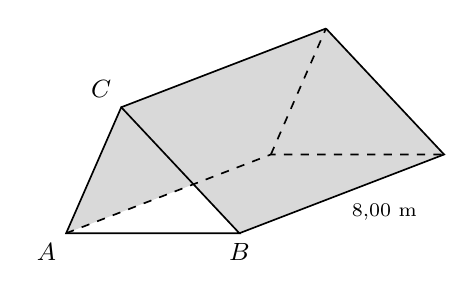
\begin{tikzpicture}[line width=0.6pt,baseline=(current bounding box.north)]\fill[black!15] (0.00,0.00) -- (0.70,1.60) -- (3.30,2.60) -- (2.60,1.00) -- cycle;\fill[black!15] (2.20,0.00) -- (0.70,1.60) -- (3.30,2.60) -- (4.80,1.00) -- cycle;\draw (0.00,0.00) -- (2.20,0.00) -- (0.70,1.60) -- cycle;\draw (3.30,2.60) -- (4.80,1.00) -- (2.20,0.00); \draw[dashed] (0.00,0.00) -- (2.60,1.00) -- (4.80,1.00);\draw (0.70,1.60) -- (3.30,2.60); \draw[dashed] (2.60,1.00) -- (3.30,2.60);\node[font=\small,anchor=north east] at (0.00,0.00) {$A$};\node[font=\small,anchor=north] at (2.20,0.00) {$B$};\node[font=\small,anchor=south east] at (0.70,1.60) {$C$};\path (2.20,0.00) -- node[font=\scriptsize,below right] {8,00 m} (4.80,1.00);\end{tikzpicture}\par
\rechenplatz{4}
\fusshilfe{\mbox{62:~$\approx$ 7,00 m; $\approx$ 92 m²}}
\end{pfaufg}

\pfstufekopf[sseiteberechnensinuss]{Seite berechnen (Sinussatz)}{in 2 der letzten 5 Prüfungen}
\pfgruppe{}
\begin{pfaufg}{}{63.}{}
Im Dreieck $ABC$ ist $\alpha = 47^\circ$ und $\beta = 62^\circ$. Die Seite $a$ ist gegeben. Kreuze an, womit du die Seite $b$ berechnest. 
\pfkreuzzeile{sin, cos, tan}\pfkreuzzeile{Sinussatz}
\fusshilfe{\mbox{63:~Sinussatz}}
\end{pfaufg}
\pfgruppe{}
\begin{pfaufg}{P10 ’18}{64.}{}
Lea will die Höhe eines Berges bestimmen. Auf der Bergspitze C steht eine 12,0 m hohe Aussichtsplattform, ihre Spitze heißt D. Lea peilt von einem Punkt A aus, der 1,5 m über dem Boden liegt. Zur Bergspitze C misst sie gegenüber der Waagerechten 30°, zur Plattformspitze D 35°. B ist der Punkt senkrecht unter C auf der Höhe von A; bei B ist ein rechter Winkel. Der Winkel zwischen den beiden Peillinien heißt $\gamma$, der Winkel bei D im Dreieck ACD heißt $\delta$. Gegeben: AC = 112,8 m. Ermittle die Höhe des Berges über dem Boden. Gib an, wie hoch über dem Boden die Spitze D der Plattform liegt.
\par\smallskip\noindent \begin{tikzpicture}[line width=0.6pt,baseline=(current bounding box.north)]\draw[dashed] (-0.4,0) -- (6.2,0);\draw (0,0) -- (0.00,0.60);\draw (0.00,0.60) -- (5.50,0.60) -- (5.50,4.20);\draw (0.00,0.60) -- (5.50,3.10); \draw (0.00,0.60) -- (5.50,4.20);\draw[line width=1.2pt] (5.50,3.10) -- (5.50,4.20);\node[font=\small,anchor=east] at (0.00,0.60) {$A$};\node[font=\small,anchor=north west] at (5.50,0.60) {$B$};\node[font=\small,anchor=west] at (5.50,3.10) {$C$};\node[font=\small,anchor=south] at (5.50,4.20) {$D$};\path (0.00,0.00) -- node[font=\scriptsize,left] {1,5 m} (0.00,0.60);\path (5.50,3.10) -- node[font=\scriptsize,right] {12,0 m} (5.50,4.20);\draw[line width=0.4pt] (0.00,0.60) ++(0:1.6) arc (0:24.4:1.6);\node[font=\scriptsize,fill=white,inner sep=0.5pt] at ($(0.00,0.60)+(12.2:1.9000000000000001)$) {30°};\draw[line width=0.4pt] (0.00,0.60) ++(24.4:2.4) arc (24.4:33.2:2.4);\node[font=\scriptsize,fill=white,inner sep=0.5pt] at ($(0.00,0.60)+(28.8:2.6999999999999997)$) {$\gamma$};\draw[line width=0.4pt] (5.50,0.85) -- (5.25,0.85) -- (5.25,0.60);\draw[line width=0.4pt] (5.50,4.20) ++(213.2:0.6) arc (213.2:270:0.6);\node[font=\scriptsize,fill=white,inner sep=0.5pt] at ($(5.50,4.20)+(241.6:0.8999999999999999)$) {$\delta$};\draw[line width=0.4pt] (0.00,0.60) ++(0:3.4) arc (0:33.2:3.4);\node[font=\scriptsize,fill=white,inner sep=0.5pt] at ($(0.00,0.60)+(16.6:3.6999999999999997)$) {35°};\node[font=\scriptsize,mbgrau,anchor=north west] at ([yshift=-2pt]current bounding box.south west) {nicht maßstabsgerecht};\end{tikzpicture}\par
\rechenplatz{3}
\fusshilfe{\mbox{64:~57,9 m; 69,9 m}}
\end{pfaufg}
\pfgruppe{}
\begin{pfaufg}{P10 ’15}{\llap{\textasteriskcentered\,}65.}{}
Gegeben ist ein Drachenviereck ABCD. Die Diagonale AC ist senkrecht (A unten, C oben), die Diagonale BD waagerecht (D links, B rechts); beide schneiden sich in E im rechten Winkel. Die Seite AD ist 4,1 cm lang. Im Dreieck ABD ist der Winkel bei A 123° und der Winkel bei B 36° groß; der Winkel bei D heißt $\delta$. Berechne die Länge der Diagonale BD.
\par\smallskip\noindent \begin{tikzpicture}[x=0.750cm,y=0.750cm,line width=0.6pt,baseline=(current bounding box.north)]\draw (3.000,0.000) -- (6.000,1.750) -- (3.000,3.500) -- (-2.000,1.750) -- cycle;\draw[] (3.000,0.000) -- (3.000,1.750);\draw[] (3.000,1.750) -- (3.000,3.500);\draw[] (6.000,1.750) -- (3.000,1.750);\draw[] (3.000,1.750) -- (-2.000,1.750);\draw[line width=0.4pt] (3.000,1.377) -- (3.373,1.377) -- (3.373,1.750);\fill (3.187,1.563) circle (0.6pt);\draw[line width=0.4pt] (3.484,0.282) arc (30.26:160.71:0.560);\node[font=\scriptsize,inner sep=0.5pt,fill=white] at (2.883,1.221) {123°};\draw[line width=0.4pt] (5.000,1.750) arc (180.00:210.26:1.000);\node[font=\scriptsize,inner sep=0.5pt,fill=white] at (4.391,1.315) {36°};\draw[line width=0.4pt] (-1.056,1.420) arc (-19.29:0.00:1.000);\node[font=\scriptsize,inner sep=0.5pt,fill=white] at (-0.593,1.511) {$\delta$};\node[font=\scriptsize,anchor=north,inner sep=2pt] at (0.500,0.875) {4,1 cm};\node[font=\small,inner sep=1pt] at (3.110,3.885) {$C$};\node[font=\small,inner sep=1pt] at (3.110,-0.385) {$A$};\node[font=\small,inner sep=1pt] at (-2.400,1.750) {$D$};\node[font=\small,inner sep=1pt] at (6.400,1.750) {$B$};\node[font=\small,inner sep=1pt] at (3.400,1.750) {$E$};\node[font=\scriptsize,mbgrau,anchor=north west] at ([yshift=-2pt]current bounding box.south west) {nicht maßstabsgerecht};\end{tikzpicture}\par
\rechenplatz{2}
\fusshilfe{\mbox{65:~BD = 4,1 · sin 123° : sin 36° $\approx$ 5,85 cm}}
\end{pfaufg}
\begin{pfaufg}{P10 ’17}{66.}{}
Ein Dachboden hat als Querschnitt das Dreieck ABC. Die Dachschräge AC ist 4,50 m lang. Der Winkel bei A beträgt 62,8°, der Winkel bei B 34,9°; der Winkel bei C heißt $\gamma$. Auf dem Boden AB steht im Punkt P eine senkrechte Wand, die genau bis zur Dachschräge BC reicht. Sie ist 1,20 m hoch. Berechne den Abstand von P bis B.
\par\smallskip\noindent \begin{tikzpicture}[x=1.000cm,y=1.000cm,line width=0.6pt,baseline=(current bounding box.north)]\draw (0.000,0.000) -- (6.000,0.000) -- (2.000,3.500) -- cycle;\draw[line width=1.2pt] (4.800,0.000) -- (4.800,1.050);\draw[line width=0.4pt] (4.800,0.280) -- (4.520,0.280) -- (4.520,0.000);\fill (4.660,0.140) circle (0.6pt);\draw[line width=0.4pt] (0.420,0.000) arc (0.00:60.26:0.420);\node[font=\scriptsize,inner sep=0.5pt,fill=white] at (0.796,0.462) {62,8°};\draw[line width=0.4pt] (5.684,0.277) arc (138.81:180.00:0.420);\node[font=\scriptsize,inner sep=0.5pt,fill=white] at (5.139,0.324) {34,9°};\draw[line width=0.4pt] (1.792,3.135) arc (-119.74:-41.19:0.420);\node[font=\scriptsize,inner sep=0.5pt,fill=white] at (2.123,2.770) {$\gamma$};\node[font=\scriptsize,anchor=west,inner sep=2pt] at (4.800,0.525) {1,20 m};\node[font=\scriptsize,anchor=east,inner sep=2pt] at (1.000,1.750) {4,50 m};\node[font=\small,inner sep=1pt] at (-0.275,-0.120) {$A$};\node[font=\small,inner sep=1pt] at (6.283,-0.099) {$B$};\node[font=\small,inner sep=1pt] at (1.918,3.788) {$C$};\node[font=\small,inner sep=1pt] at (5.063,-0.144) {$P$};\node[font=\scriptsize,mbgrau,anchor=north west] at ([yshift=-2pt]current bounding box.south west) {nicht maßstabsgerecht};\end{tikzpicture}\par
\rechenplatz{2}
\fusshilfe{\mbox{66:~PB = 1,20 : tan 34,9° $\approx$ 1,72 m}}
\end{pfaufg}
\begin{pfaufg}{P10 ’18}{\llap{\textasteriskcentered\,}67.}{}
Lea will die Höhe eines Berges bestimmen. Auf der Bergspitze C steht eine 12,0 m hohe Aussichtsplattform, ihre Spitze heißt D. Lea peilt von einem Punkt A aus, der 1,5 m über dem Boden liegt. Zur Bergspitze C misst sie gegenüber der Waagerechten 30°, zur Plattformspitze D 35°. B ist der Punkt senkrecht unter C auf der Höhe von A; bei B ist ein rechter Winkel. Der Winkel zwischen den beiden Peillinien heißt $\gamma$, der Winkel bei D im Dreieck ACD heißt $\delta$. Lea erhält für die Strecke AC 112,8 m. Bestätige diesen Wert mit einer Rechnung. Gegeben: $\gamma$ = 5°, $\delta$ = 55°.
\par\smallskip\noindent \begin{tikzpicture}[line width=0.6pt,baseline=(current bounding box.north)]\draw[dashed] (-0.4,0) -- (6.2,0);\draw (0,0) -- (0.00,0.60);\draw (0.00,0.60) -- (5.50,0.60) -- (5.50,4.20);\draw (0.00,0.60) -- (5.50,3.10); \draw (0.00,0.60) -- (5.50,4.20);\draw[line width=1.2pt] (5.50,3.10) -- (5.50,4.20);\node[font=\small,anchor=east] at (0.00,0.60) {$A$};\node[font=\small,anchor=north west] at (5.50,0.60) {$B$};\node[font=\small,anchor=west] at (5.50,3.10) {$C$};\node[font=\small,anchor=south] at (5.50,4.20) {$D$};\path (0.00,0.00) -- node[font=\scriptsize,left] {1,5 m} (0.00,0.60);\path (5.50,3.10) -- node[font=\scriptsize,right] {12,0 m} (5.50,4.20);\draw[line width=0.4pt] (0.00,0.60) ++(0:1.6) arc (0:24.4:1.6);\node[font=\scriptsize,fill=white,inner sep=0.5pt] at ($(0.00,0.60)+(12.2:1.9000000000000001)$) {30°};\draw[line width=0.4pt] (0.00,0.60) ++(24.4:2.4) arc (24.4:33.2:2.4);\node[font=\scriptsize,fill=white,inner sep=0.5pt] at ($(0.00,0.60)+(28.8:2.6999999999999997)$) {$\gamma$};\draw[line width=0.4pt] (5.50,0.85) -- (5.25,0.85) -- (5.25,0.60);\draw[line width=0.4pt] (5.50,4.20) ++(213.2:0.6) arc (213.2:270:0.6);\node[font=\scriptsize,fill=white,inner sep=0.5pt] at ($(5.50,4.20)+(241.6:0.8999999999999999)$) {$\delta$};\draw[line width=0.4pt] (0.00,0.60) ++(0:3.4) arc (0:33.2:3.4);\node[font=\scriptsize,fill=white,inner sep=0.5pt] at ($(0.00,0.60)+(16.6:3.6999999999999997)$) {35°};\node[font=\scriptsize,mbgrau,anchor=north west] at ([yshift=-2pt]current bounding box.south west) {nicht maßstabsgerecht};\end{tikzpicture}\par
\rechenplatz{2}
\fusshilfe{\mbox{67:~AC = 12 · sin 55° : sin 5° $\approx$ 112,8 m}}
\end{pfaufg}
\begin{pfaufg}{P10 ’21}{68.}{}
Gegeben ist das Viereck ABCD mit der Diagonale BD = 1500 m. Bei A ist ein rechter Winkel. Die Seite DC ist 2004 m lang. Bei D ist der Winkel zwischen DA und DB 55° groß und der Winkel zwischen DB und DC 60°. Bei B ist der Innenwinkel $\angle$ABC = 109° groß. Zeige mit einer Rechnung, dass die Strecke AB etwa 1229 m lang ist.
\par\smallskip\noindent \begin{tikzpicture}[x=0.706cm,y=0.706cm,line width=0.6pt,baseline=(current bounding box.north)]\draw (6.000,0.000) -- (6.000,3.500) -- (-2.500,4.200) -- (0.000,0.000) -- cycle;\draw[] (6.000,3.500) -- (0.000,0.000);\draw[line width=0.4pt] (6.000,0.397) -- (5.603,0.397) -- (5.603,0.000);\fill (5.802,0.198) circle (0.6pt);\draw[line width=0.4pt] (1.062,0.000) arc (0.00:30.26:1.062);\node[font=\scriptsize,inner sep=0.5pt,fill=white] at (1.709,0.462) {55°};\draw[line width=0.4pt] (0.514,0.300) arc (30.26:120.76:0.595);\node[font=\scriptsize,inner sep=0.5pt,fill=white] at (0.326,1.262) {60°};\draw[line width=0.4pt] (5.407,3.549) arc (175.29:270.00:0.595);\node[font=\scriptsize,inner sep=0.5pt,fill=white] at (5.041,2.617) {109°};\node[font=\scriptsize,anchor=north,inner sep=2pt] at (3.000,1.750) {1500 m};\node[font=\scriptsize,anchor=east,inner sep=2pt] at (-1.250,2.100) {2004 m};\node[font=\small,inner sep=1pt] at (6.375,-0.199) {$A$};\node[font=\small,inner sep=1pt] at (-2.885,4.380) {$C$};\node[font=\small,inner sep=1pt] at (6.390,3.669) {$B$};\node[font=\small,inner sep=1pt] at (-0.330,-0.268) {$D$};\node[font=\scriptsize,mbgrau,anchor=north west] at ([yshift=-2pt]current bounding box.south west) {nicht maßstabsgerecht};\end{tikzpicture}\par
\rechenplatz{2}
\fusshilfe{\mbox{68:~AB = 1500 · sin 55° $\approx$ 1228,7 m $\approx$ 1229 m}}
\end{pfaufg}
\begin{pfaufg}{P10 ’21}{69.}{}
Gegeben ist das Viereck ABCD mit der Diagonale BD = 1500 m. Bei A ist ein rechter Winkel. Die Seite DC ist 2004 m lang. Bei D ist der Winkel zwischen DA und DB 55° groß und der Winkel zwischen DB und DC 60°. Bei B ist der Innenwinkel $\angle$ABC = 109° groß. Berechne die Länge der Strecke AD.
\par\smallskip\noindent \begin{tikzpicture}[x=0.706cm,y=0.706cm,line width=0.6pt,baseline=(current bounding box.north)]\draw (6.000,0.000) -- (6.000,3.500) -- (-2.500,4.200) -- (0.000,0.000) -- cycle;\draw[] (6.000,3.500) -- (0.000,0.000);\draw[line width=0.4pt] (6.000,0.397) -- (5.603,0.397) -- (5.603,0.000);\fill (5.802,0.198) circle (0.6pt);\draw[line width=0.4pt] (1.062,0.000) arc (0.00:30.26:1.062);\node[font=\scriptsize,inner sep=0.5pt,fill=white] at (1.709,0.462) {55°};\draw[line width=0.4pt] (0.514,0.300) arc (30.26:120.76:0.595);\node[font=\scriptsize,inner sep=0.5pt,fill=white] at (0.326,1.262) {60°};\draw[line width=0.4pt] (5.407,3.549) arc (175.29:270.00:0.595);\node[font=\scriptsize,inner sep=0.5pt,fill=white] at (5.041,2.617) {109°};\node[font=\scriptsize,anchor=north,inner sep=2pt] at (3.000,1.750) {1500 m};\node[font=\scriptsize,anchor=east,inner sep=2pt] at (-1.250,2.100) {2004 m};\node[font=\small,inner sep=1pt] at (6.375,-0.199) {$A$};\node[font=\small,inner sep=1pt] at (-2.885,4.380) {$C$};\node[font=\small,inner sep=1pt] at (6.390,3.669) {$B$};\node[font=\small,inner sep=1pt] at (-0.330,-0.268) {$D$};\node[font=\scriptsize,mbgrau,anchor=north west] at ([yshift=-2pt]current bounding box.south west) {nicht maßstabsgerecht};\end{tikzpicture}\par
\rechenplatz{2}
\fusshilfe{\mbox{69:~AD = 1500 · cos 55° $\approx$ 860,4 m}}
\end{pfaufg}
\begin{pfaufg}{P10 ’22}{70.}{}
Gegeben ist ein Dreieck ABC, das nicht rechtwinklig ist. Die Höhe $h_c$ von C auf die Seite AB ist etwa 7,4 m lang; ihr Fußpunkt heißt D. Die Seite b = AC ist 14,1 m lang, der Winkel bei B ist 52° groß. Der Winkel bei C zwischen AC und der Höhe heißt $\gamma_1$. Berechne die Länge der Seite a.
\par\smallskip\noindent \begin{tikzpicture}[x=1.000cm,y=1.000cm,line width=0.6pt,baseline=(current bounding box.north)]\draw (0.000,0.000) -- (6.000,0.000) -- (3.000,3.500) -- cycle;\draw[dashed] (3.000,3.500) -- (3.000,0.000);\draw[line width=0.4pt] (3.000,0.280) -- (2.720,0.280) -- (2.720,0.000);\fill (2.860,0.140) circle (0.6pt);\draw[line width=0.4pt] (0.420,0.000) arc (0.00:49.40:0.420);\node[font=\scriptsize,inner sep=0.5pt,fill=white] at (0.672,0.309) {$\alpha$};\draw[line width=0.4pt] (5.727,0.319) arc (130.60:180.00:0.420);\node[font=\scriptsize,inner sep=0.5pt,fill=white] at (5.164,0.384) {52°};\draw[line width=0.4pt] (3.000,3.080) arc (-90.00:0.00:0.420);\node[font=\scriptsize,inner sep=0.5pt,fill=white] at (3.523,2.977) {$\gamma_1$};\node[font=\scriptsize,anchor=west,inner sep=2pt] at (3.000,1.750) {$h_c$};\node[font=\scriptsize,anchor=east,inner sep=2pt] at (1.500,1.750) {b = 14,1 m};\node[font=\scriptsize,anchor=west,inner sep=2pt] at (4.500,1.750) {a};\node[font=\small,inner sep=1pt] at (-0.280,-0.109) {$A$};\node[font=\small,inner sep=1pt] at (6.280,-0.109) {$B$};\node[font=\small,inner sep=1pt] at (3.000,3.800) {$C$};\node[font=\small,inner sep=1pt] at (3.000,-0.300) {$D$};\node[font=\scriptsize,mbgrau,anchor=north west] at ([yshift=-2pt]current bounding box.south west) {nicht maßstabsgerecht};\end{tikzpicture}\par
\rechenplatz{2}
\fusshilfe{\mbox{70:~a = 7,4 : sin 52° $\approx$ 9,4 m}}
\end{pfaufg}
\begin{pfaufg}{P10 ’25}{\llap{\textasteriskcentered\,}71.}{}
Am Hinterausgang sollen zwei Stufen mit einer mobilen Rampe y überwunden werden. Vom Fuß der Rampe bis zum Fuß der Treppe sind es waagerecht 160 cm. Die Rampe steigt unter 5° an. Eine gedachte Linie vom Fuß der Treppe zur oberen Stufenkante bildet mit dem Boden (zur Rampe hin) einen Winkel von 141°. Berechne die Länge y der Rampe.
\par\smallskip\noindent \begin{tikzpicture}[line width=0.6pt,baseline=(current bounding box.north)]\fill[black!20] (5.0,0) rectangle (5.7,0.5); \fill[black!20] (5.7,0) rectangle (6.4,1.0);\draw (-0.3,0) -- (7,0); \draw (0.00,0.00) -- (6.40,1.00);\draw[dashed] (5.00,0.00) -- (6.40,1.00);\node[font=\scriptsize,anchor=north] at (0,0) {Rampenfuß};\node[font=\scriptsize,anchor=north] at (5,0) {Treppenfuß};\node[font=\scriptsize,anchor=south] at (6.4,1.0) {Stufenkante};\path (0.00,0.00) -- node[font=\scriptsize,below=8pt] {160 cm} (5.00,0.00);\path (0.00,0.00) -- node[font=\scriptsize,above] {$y$} (6.40,1.00);\draw[line width=0.4pt] (0.00,0.00) ++(0:1.4) arc (0:8.9:1.4);\node[font=\scriptsize,fill=white,inner sep=0.5pt] at ($(0.00,0.00)+(4.45:1.7)$) {5°};\draw[line width=0.4pt] (5.00,0.00) ++(35.5:0.35) arc (35.5:180:0.35);\node[font=\scriptsize,fill=white,inner sep=0.5pt] at ($(5.00,0.00)+(107.75:0.6499999999999999)$) {141°};\node[font=\scriptsize,mbgrau,anchor=north west] at ([yshift=-2pt]current bounding box.south west) {nicht maßstabsgerecht};\end{tikzpicture}\par
\rechenplatz{3}
\fusshilfe{\mbox{71:~y = 160 · sin 141° : sin 34° $\approx$ 180,1 cm}}
\end{pfaufg}
\begin{pfaufg}{P10 ’14}{\llap{\textasteriskcentered\,}72.}{}
Von einer Jugendherberge J führt ein Weg zu einem Forsthaus F, 2800 m lang. Vom Forsthaus führt ein gerader Weg über eine Badestelle zu einem Restaurant R; die Badestelle liegt 2500 m vor dem Restaurant. Direkt von der Jugendherberge zum Restaurant gibt es ebenfalls einen geraden Weg. Am Forsthaus schließen die Wege nach J und nach R einen Winkel von 60° ein, am Restaurant die Wege nach F und nach J einen Winkel von 50°. Eine Gruppe läuft von der Jugendherberge zuerst zum Restaurant und dann weiter zur Badestelle. Berechne die Länge dieses Weges.
\par\smallskip\noindent \begin{tikzpicture}[x=1.000cm,y=1.000cm,line width=0.6pt,baseline=(current bounding box.north)]\draw (0.000,1.750) -- (6.000,3.500) -- (6.000,0.000) -- cycle;\draw[line width=0.4pt] (0.720,1.540) arc (-16.26:16.26:0.750);\node[font=\scriptsize,inner sep=0.5pt,fill=white] at (1.250,1.750) {60°};\draw[line width=0.4pt] (6.000,0.420) arc (90.00:163.74:0.420);\node[font=\scriptsize,inner sep=0.5pt,fill=white] at (5.448,0.736) {50°};\node[font=\scriptsize,anchor=south,inner sep=2pt] at (3.000,2.625) {2800 m};\node[font=\scriptsize,anchor=north,inner sep=2pt] at (1.125,1.422) {1,5 km};\node[font=\scriptsize,anchor=north,inner sep=2pt] at (4.125,0.547) {2500 m};\node[font=\small,inner sep=1pt] at (-0.300,1.750) {$F$};\node[font=\small,inner sep=1pt] at (6.226,3.698) {$J$};\node[font=\small,inner sep=1pt] at (6.226,-0.198) {$R$};\node[font=\scriptsize,inner sep=1pt] at (2.340,1.401) {Badestelle};\fill (2.250,1.094) circle (1.4pt);\node[font=\scriptsize,mbgrau,anchor=north west] at ([yshift=-2pt]current bounding box.south west) {nicht maßstabsgerecht};\end{tikzpicture}\par
\rechenplatz{3}
\fusshilfe{\mbox{72:~$\approx$ 5,67 km)}}
\end{pfaufg}
\begin{pfaufg}{P10 ’16}{\llap{\textasteriskcentered\,}73.}{}
An einem Fluss liegen der Bioladen C, eine Brücke D und eine Anlegestelle B auf einer Geraden am Ufer, in dieser Reihenfolge. Von einem Ausflugslokal A führt ein 920 m langer Weg zum Bioladen; vom Bioladen bis zur Brücke sind es 541 m. Die Strecke AD steht senkrecht auf dem Ufer. Am Bioladen ist der Winkel zwischen den Wegen nach A und nach D 54° groß, am Lokal der Winkel zwischen den Richtungen nach C und nach B 70°. Auch von der Anlegestelle B soll ein neuer Weg direkt zur Brücke D führen. Ermittle die Länge von BD. Gegeben: AD $\approx$ 744 m.
\par\smallskip\noindent \begin{tikzpicture}[line width=0.6pt,baseline=(current bounding box.north)]\draw (-0.6,3.12) -- (6.4,1.72);\draw (2.49,-0.15) -- (0.00,3.00);\draw (2.49,-0.15) -- (5.60,1.88);\draw[dashed] (2.49,-0.15) -- (3.00,2.40);\node[font=\small,anchor=south] at (0.00,3.00) {$C$};\node[font=\small,anchor=south] at (3.00,2.40) {$D$};\node[font=\small,anchor=south] at (5.60,1.88) {$B$};\node[font=\small,anchor=north] at (2.49,-0.15) {$A$};\path (2.49,-0.15) -- node[font=\scriptsize,left] {920 m} (0.00,3.00);\path (0.00,3.00) -- node[font=\scriptsize,above] {541 m} (3.00,2.40);\draw[line width=0.4pt] (0.00,3.00) ++(308.33096706931855:0.55) arc (308.33096706931855:348.69006752597977:0.55);\node[font=\scriptsize,fill=white,inner sep=0.5pt] at ($(0.00,3.00)+(328.51051729764913:0.8500000000000001)$) {54°};\draw[line width=0.4pt] (2.49,-0.15) ++(33.128308197129584:0.7) arc (33.128308197129584:128.33096706931855:0.7);\node[font=\scriptsize,fill=white,inner sep=0.5pt] at ($(2.49,-0.15)+(80.72963763322406:1.0)$) {70°};\draw[line width=0.4pt] (2.95,2.15) -- (3.20,2.11) -- (3.25,2.35);\node[font=\scriptsize,mbgrau,anchor=west] at (6.4,1.72) {Ufer};\node[font=\scriptsize,mbgrau,anchor=north west] at ([yshift=-2pt]current bounding box.south west) {nicht maßstabsgerecht};\end{tikzpicture}\par
\rechenplatz{3}
\fusshilfe{\mbox{73:~BD = √553 719 · tan 34° $\approx$ 502 m}}
\end{pfaufg}
\begin{pfaufg}{P10 ’24}{\llap{\textasteriskcentered\,}74.}{}
Eine Seilbahn führt vom Ort B im Tal zum Ort A auf einem Berg. F liegt senkrecht unter A auf der Höhe von B; bei F ist ein rechter Winkel. FB ist 255 m lang, die Seilbahnstrecke AB 384 m. Eine zweite Seilbahn verbindet B mit dem Ort C auf einem anderen Berg. Bei B heißt der Winkel zwischen BF und BA $\beta_1$, der Winkel zwischen BA und BC $\beta_2$; bei A heißt der Winkel zwischen AB und AC $\alpha$. Für die zweite Seilbahn gilt: $\alpha$ = 38° und $\beta_2$ = 108°. Berechne die Länge der Strecke BC.
\par\smallskip\noindent \begin{tikzpicture}[x=1.000cm,y=1.000cm,line width=0.6pt,baseline=(current bounding box.north)]\draw (0.000,3.500) -- (0.000,0.000) -- (6.000,0.000) -- cycle;\draw[] (6.000,3.500) -- (0.000,3.500);\draw[] (6.000,3.500) -- (6.000,0.000);\draw[line width=0.4pt] (0.280,0.000) -- (0.280,0.280) -- (0.000,0.280);\fill (0.140,0.140) circle (0.6pt);\draw[line width=0.4pt] (5.352,0.378) arc (149.74:180.00:0.750);\node[font=\scriptsize,inner sep=0.5pt,fill=white] at (4.967,0.279) {$\beta_1$};\draw[line width=0.4pt] (6.000,0.420) arc (90.00:149.74:0.420);\node[font=\scriptsize,inner sep=0.5pt,fill=white] at (5.631,0.642) {$\beta_2$};\draw[line width=0.4pt] (0.000,3.080) arc (-90.00:-30.26:0.420);\node[font=\scriptsize,inner sep=0.5pt,fill=white] at (0.369,2.858) {$\alpha$};\node[font=\scriptsize,anchor=north,inner sep=2pt] at (3.000,0.000) {255 m};\node[font=\scriptsize,anchor=south,inner sep=2pt] at (3.000,1.750) {384 m};\node[font=\small,inner sep=1pt] at (-0.195,3.728) {$A$};\node[font=\small,inner sep=1pt] at (6.259,3.651) {$C$};\node[font=\small,inner sep=1pt] at (-0.259,-0.151) {$F$};\node[font=\small,inner sep=1pt] at (6.288,-0.084) {$B$};\node[font=\scriptsize,mbgrau,anchor=north west] at ([yshift=-2pt]current bounding box.south west) {nicht maßstabsgerecht};\end{tikzpicture}\par
\rechenplatz{3}
\fusshilfe{\mbox{74:~BC = 384 · sin 38° : sin 34° $\approx$ 422,8 m}}
\end{pfaufg}
\pfgruppe{}
\begin{pfaufg}{P10 ’23}{75.}{}
Gegeben ist das Dreieck ABC. Der Punkt F liegt auf der Seite AC, und BF steht senkrecht auf AC. Die Seite AB ist 131,5 cm lang. Bei B teilt BF den Winkel in 65° (zwischen BC und BF) und 45° (zwischen BF und BA). Der Winkel bei A ist 45° groß. Weise nach, dass BF und AF jeweils etwa 93,0 cm lang sind. Berechne die Länge der Strecke BC.
\par\smallskip\noindent \begin{tikzpicture}[x=1.000cm,y=1.000cm,line width=0.6pt,baseline=(current bounding box.north)]\begin{scope}\clip (6.000,0.000) -- (3.000,3.500) -- (3.000,0.000) -- cycle;\foreach \i in {-40,...,40}{\draw[line width=0.3pt] (\i*0.25-6,-6) -- ++(14,14);}\end{scope}\draw (0.000,0.000) -- (6.000,0.000) -- (3.000,3.500) -- cycle;\draw[] (3.000,3.500) -- (3.000,0.000);\draw[line width=0.4pt] (3.000,0.280) -- (2.720,0.280) -- (2.720,0.000);\fill (2.860,0.140) circle (0.6pt);\draw[line width=0.4pt] (2.727,3.181) arc (-130.60:-90.00:0.420);\node[font=\scriptsize,inner sep=0.5pt,fill=white] at (2.681,2.637) {65°};\draw[line width=0.4pt] (3.000,3.080) arc (-90.00:-49.40:0.420);\node[font=\scriptsize,inner sep=0.5pt,fill=white] at (3.319,2.637) {45°};\draw[line width=0.4pt] (5.727,0.319) arc (130.60:180.00:0.420);\node[font=\scriptsize,inner sep=0.5pt,fill=white] at (5.164,0.384) {45°};\node[font=\scriptsize,anchor=west,inner sep=2pt] at (4.500,1.750) {131,5 cm};\node[font=\small,inner sep=1pt] at (-0.280,-0.109) {$C$};\node[font=\small,inner sep=1pt] at (6.280,-0.109) {$A$};\node[font=\small,inner sep=1pt] at (3.000,3.800) {$B$};\node[font=\small,inner sep=1pt] at (3.000,-0.300) {$F$};\fill (3.000,0.000) circle (1.4pt);\node[font=\scriptsize,mbgrau,anchor=north west] at ([yshift=-2pt]current bounding box.south west) {nicht maßstabsgerecht};\end{tikzpicture}\par
\rechenplatz{3}
\fusshilfe{\mbox{75:~65,75√2 $\approx$ 93,0 cm; $\approx$ 220,0 cm}}
\end{pfaufg}
\pfgruppe{}
\begin{pfaufg}{P10 ’20}{\llap{\textasteriskcentered\,}76.}{}
Im Dreieck DEF ist DF = 4 m und FE = 11 m. Der Winkel bei F ist 115° groß, der Winkel bei E 16°. Der Punkt P liegt auf der Strecke DE, und PE ist 10 m lang. Berechne die Länge der Strecke DP.
\par\smallskip\noindent \begin{tikzpicture}[x=1.000cm,y=1.000cm,line width=0.6pt,baseline=(current bounding box.north)]\draw (0.000,0.000) -- (6.000,1.750) -- (0.000,3.500) -- cycle;\draw[line width=0.4pt] (0.000,3.080) arc (-90.00:-16.26:0.420);\node[font=\scriptsize,inner sep=0.5pt,fill=white] at (0.552,2.764) {115°};\draw[line width=0.4pt] (5.280,1.960) arc (163.74:196.26:0.750);\node[font=\scriptsize,inner sep=0.5pt,fill=white] at (4.750,1.750) {16°};\node[font=\scriptsize,anchor=east,inner sep=2pt] at (0.000,1.750) {4 m};\node[font=\scriptsize,anchor=south,inner sep=2pt] at (3.000,2.625) {11 m};\node[font=\small,inner sep=1pt] at (-0.226,-0.198) {$D$};\node[font=\small,inner sep=1pt] at (6.300,1.750) {$E$};\node[font=\small,inner sep=1pt] at (-0.226,3.698) {$F$};\node[font=\small,inner sep=1pt] at (1.051,0.090) {$P$};\fill (1.200,0.350) circle (1.4pt);\node[font=\scriptsize,mbgrau,anchor=north west] at ([yshift=-2pt]current bounding box.south west) {nicht maßstabsgerecht};\end{tikzpicture}\par
\rechenplatz{4}
\fusshilfe{\mbox{76:~DP = 11 · sin 115° : sin 49° $-$ 10 $\approx$ 3,2 m}}
\end{pfaufg}
\pfgruppe{}
\begin{pfaufg}{P10 ’21}{\llap{\textasteriskcentered\,}77.}{}
Gegeben ist das Viereck ABCD mit der Diagonale BD = 1500 m. Bei A ist ein rechter Winkel. Die Seite DC ist 2004 m lang. Bei D ist der Winkel zwischen DA und DB 55° groß und der Winkel zwischen DB und DC 60°. Bei B ist der Innenwinkel $\angle$ABC = 109° groß. Jemand behauptet: „BC und DC sind gleich lang.“ Prüfe mit einer Rechnung, ob das stimmt.
\par\smallskip\noindent \begin{tikzpicture}[x=0.706cm,y=0.706cm,line width=0.6pt,baseline=(current bounding box.north)]\draw (6.000,0.000) -- (6.000,3.500) -- (-2.500,4.200) -- (0.000,0.000) -- cycle;\draw[] (6.000,3.500) -- (0.000,0.000);\draw[line width=0.4pt] (6.000,0.397) -- (5.603,0.397) -- (5.603,0.000);\fill (5.802,0.198) circle (0.6pt);\draw[line width=0.4pt] (1.062,0.000) arc (0.00:30.26:1.062);\node[font=\scriptsize,inner sep=0.5pt,fill=white] at (1.709,0.462) {55°};\draw[line width=0.4pt] (0.514,0.300) arc (30.26:120.76:0.595);\node[font=\scriptsize,inner sep=0.5pt,fill=white] at (0.326,1.262) {60°};\draw[line width=0.4pt] (5.407,3.549) arc (175.29:270.00:0.595);\node[font=\scriptsize,inner sep=0.5pt,fill=white] at (5.041,2.617) {109°};\node[font=\scriptsize,anchor=north,inner sep=2pt] at (3.000,1.750) {1500 m};\node[font=\scriptsize,anchor=east,inner sep=2pt] at (-1.250,2.100) {2004 m};\node[font=\small,inner sep=1pt] at (6.375,-0.199) {$A$};\node[font=\small,inner sep=1pt] at (-2.885,4.380) {$C$};\node[font=\small,inner sep=1pt] at (6.390,3.669) {$B$};\node[font=\small,inner sep=1pt] at (-0.330,-0.268) {$D$};\node[font=\scriptsize,mbgrau,anchor=north west] at ([yshift=-2pt]current bounding box.south west) {nicht maßstabsgerecht};\end{tikzpicture}\par
\rechenplatz{4}
\fusshilfe{\mbox{77:~$\approx$ 1805,5 m; 2004 m)}}
\end{pfaufg}
\pfgruppe{}
\begin{pfaufg}{P10 ’19}{\llap{\textasteriskcentered\,}78.}{}
Ein viertes Kind, Deniz, steht bei D. Es entsteht das Viereck ABCD mit rechtem Winkel bei B. Die Diagonale AC ist 9 m lang. Der Winkel zwischen AB und AC beträgt 64°, der Winkel bei C zwischen CB und CD 86° und der Winkel bei D 80°. Berechne den Abstand zwischen Amir (A) und Deniz (D).
\par\smallskip\noindent \begin{tikzpicture}[x=1.000cm,y=1.000cm,line width=0.6pt,baseline=(current bounding box.north)]\draw (0.000,3.500) -- (0.000,0.000) -- (6.000,0.000) -- (6.000,3.500) -- cycle;\draw[dashed] (0.000,3.500) -- (6.000,0.000);\draw[line width=0.4pt] (0.280,0.000) -- (0.280,0.280) -- (0.000,0.280);\fill (0.140,0.140) circle (0.6pt);\draw[line width=0.4pt] (0.000,3.080) arc (-90.00:-30.26:0.420);\node[font=\scriptsize,inner sep=0.5pt,fill=white] at (0.458,2.702) {64°};\draw[line width=0.4pt] (6.000,0.420) arc (90.00:180.00:0.420);\node[font=\scriptsize,inner sep=0.5pt,fill=white] at (5.349,0.651) {86°};\draw[line width=0.4pt] (5.580,3.500) arc (180.00:270.00:0.420);\node[font=\scriptsize,inner sep=0.5pt,fill=white] at (5.349,2.849) {80°};\node[font=\scriptsize,anchor=south,inner sep=2pt] at (3.000,1.750) {9 m};\node[font=\small,inner sep=1pt] at (-0.259,-0.151) {$B$};\node[font=\small,inner sep=1pt] at (6.259,-0.151) {$C$};\node[font=\small,inner sep=1pt] at (6.259,3.651) {$D$};\node[font=\small,inner sep=1pt] at (-0.259,3.651) {$A$};\node[font=\scriptsize,mbgrau,anchor=north west] at ([yshift=-2pt]current bounding box.south west) {nicht maßstabsgerecht};\end{tikzpicture}\par
\rechenplatz{4}
\fusshilfe{\mbox{78:~AD = 9 · sin 60° : sin 80° $\approx$ 7,9 m}}
\end{pfaufg}
\pfgruppe{}
\begin{pfaufg}{P10 ’17}{\llap{\textasteriskcentered\,}79.}{}
Ein Dachboden hat als Querschnitt das Dreieck ABC. Die Dachschräge AC ist 4,50 m lang. Der Winkel bei A beträgt 62,8°, der Winkel bei B 34,9°; der Winkel bei C heißt $\gamma$. Die beiden Dachflächen über AC und über BC sollen gedämmt werden; der Dachboden ist 8,00 m lang. Berechne die Länge der Dachschräge BC. Berechne, wie viele Quadratmeter Dachfläche zu dämmen sind.
\par\smallskip\noindent \begin{tikzpicture}[line width=0.6pt,baseline=(current bounding box.north)]\fill[black!15] (0.00,0.00) -- (0.70,1.60) -- (3.30,2.60) -- (2.60,1.00) -- cycle;\fill[black!15] (2.20,0.00) -- (0.70,1.60) -- (3.30,2.60) -- (4.80,1.00) -- cycle;\draw (0.00,0.00) -- (2.20,0.00) -- (0.70,1.60) -- cycle;\draw (3.30,2.60) -- (4.80,1.00) -- (2.20,0.00); \draw[dashed] (0.00,0.00) -- (2.60,1.00) -- (4.80,1.00);\draw (0.70,1.60) -- (3.30,2.60); \draw[dashed] (2.60,1.00) -- (3.30,2.60);\node[font=\small,anchor=north east] at (0.00,0.00) {$A$};\node[font=\small,anchor=north] at (2.20,0.00) {$B$};\node[font=\small,anchor=south east] at (0.70,1.60) {$C$};\path (2.20,0.00) -- node[font=\scriptsize,below right] {8,00 m} (4.80,1.00);\end{tikzpicture}\par
\rechenplatz{4}
\fusshilfe{\mbox{79:~$\approx$ 7,00 m; $\approx$ 92 m²}}
\end{pfaufg}

\par\Needspace*{0.55\textheight}\pfstufekopf[serkennen1]{Was ist gesucht?}{}
\begin{pfaufg}{}{80.}{}
Was ist gesucht? Kreuze an. Rechne nicht.
\par\smallskip\noindent \begingroup\renewcommand{\arraystretch}{1.4}\begin{tabular}{|>{\raggedright\arraybackslash}p{4.3cm}|>{\centering\arraybackslash\hyphenpenalty=0}p{1.55cm}|>{\centering\arraybackslash\hyphenpenalty=0}p{1.55cm}|>{\centering\arraybackslash\hyphenpenalty=0}p{1.55cm}|>{\centering\arraybackslash\hyphenpenalty=0}p{1.55cm}|}\hline  & {\scriptsize\hspace{0pt}Pythagoras} & {\scriptsize\hspace{0pt}Winkelfunktion} & {\scriptsize\hspace{0pt}Seite berechnen} & {\scriptsize\hspace{0pt}Winkel} \\ \hline Berechne die Länge der Seite b. & $\square$ & $\square$ & $\square$ & $\square$ \\ \hline Berechne die Größe des Winkels $\alpha$. & $\square$ & $\square$ & $\square$ & $\square$ \\ \hline Im Dreieck ACD ist CD = 12 m, $\gamma$ = 5° und $\delta$ = 55°. Wie lang ist AC? & $\square$ & $\square$ & $\square$ & $\square$ \\ \hline Berechne das Maß des Winkels MSC in der Pyramide. & $\square$ & $\square$ & $\square$ & $\square$ \\ \hline Berechne die Länge der Schenkel. & $\square$ & $\square$ & $\square$ & $\square$ \\ \hline Bestimme rechnerisch die Größe des Winkels $\alpha$. & $\square$ & $\square$ & $\square$ & $\square$ \\ \hline\end{tabular}\endgroup\par
\end{pfaufg}
\pfstufekopf[swinkelsumme]{Winkelsumme}{in 5 der letzten 5 Prüfungen}
\pfgruppe{}
\begin{pfaufg}{}{81.}{}
Die Figur zeigt ein Dreieck mit den Seiten a = 4 cm, b = 4 cm und c = 6 cm. Markiere gleich lange Seiten oder den rechten Winkel. Kreuze dann an, welche Art von Dreieck es ist. 
\pfkreuzzeile{gleichseitig}\pfkreuzzeile{gleichschenklig}\pfkreuzzeile{ungleichseitig}
\par\smallskip\noindent \dreieck{(0,0)}{(6,0)}{(3,2.65)}{a}{b}{c}{\alpha}{\beta}{\gamma}\par
\fusshilfe{\mbox{81:~gleichschenklig}}
\end{pfaufg}
\begin{pfaufg}{}{82.}{}
Die Figur zeigt zwei Geraden, die sich kreuzen. Kreuze an, wie $\alpha$ und $\gamma$ zueinander liegen. 
\pfkreuzzeile{Scheitelwinkel}\pfkreuzzeile{Nebenwinkel}\pfkreuzzeile{Stufenwinkel}\pfkreuzzeile{Wechselwinkel}
\par\smallskip\noindent \geradenkreuzung{55}{\alpha}{\beta}{\gamma}{\delta}\par
\fusshilfe{\mbox{82:~Scheitelwinkel}}
\end{pfaufg}
\pfgruppe{}
\begin{pfaufg}{P10 ’26}{83.}{}
Im abgebildeten Parallelogramm ist ein Winkel 75° groß. Bestimme den Winkel $\beta$.
\par\smallskip\noindent \begin{tikzpicture}[x=0.938cm,y=0.938cm,line width=0.6pt,baseline=(current bounding box.north)]\draw (0.000,0.000) -- (5.000,0.000) -- (6.400,2.400) -- (1.400,2.400) -- cycle;\draw[line width=0.4pt] (0.448,0.000) arc (0.00:59.74:0.448);\node[font=\scriptsize,inner sep=0.5pt,fill=white] at (0.851,0.489) {75°};\draw[line width=0.4pt] (5.226,0.387) arc (59.74:180.00:0.448);\node[font=\scriptsize,inner sep=0.5pt,fill=white] at (4.607,0.684) {$\beta$};\node[font=\scriptsize,mbgrau,anchor=north west] at ([yshift=-2pt]current bounding box.south west) {nicht maßstabsgerecht};\end{tikzpicture}\par
\rechenplatz{1}
\fusshilfe{\mbox{83:~$\beta$ = 105°}}
\end{pfaufg}
\pfgruppe{}
\begin{pfaufg}{P10 ’21}{84.}{}
Bestimme die Größe des fehlenden Winkels $\alpha$ im abgebildeten Trapez.
\par\smallskip\noindent \begin{tikzpicture}[x=1.000cm,y=1.000cm,line width=0.6pt,baseline=(current bounding box.north)]\draw (1.700,0.000) -- (4.300,0.000) -- (6.000,1.674) -- (0.000,1.674) -- cycle;\draw[line width=0.4pt] (0.299,1.379) arc (-44.56:0.00:0.420);\node[font=\scriptsize,inner sep=0.5pt,fill=white] at (0.685,1.394) {$\alpha$};\draw[line width=0.4pt] (5.580,1.674) arc (180.00:224.56:0.420);\node[font=\scriptsize,inner sep=0.5pt,fill=white] at (5.149,1.325) {50°};\draw[line width=0.4pt] (2.120,0.000) arc (0.00:135.44:0.420);\node[font=\scriptsize,inner sep=0.5pt,fill=white] at (2.049,0.851) {140°};\draw[line width=0.4pt] (4.599,0.295) arc (44.56:180.00:0.420);\node[font=\scriptsize,inner sep=0.5pt,fill=white] at (3.951,0.851) {130°};\node[font=\scriptsize,mbgrau,anchor=north west] at ([yshift=-2pt]current bounding box.south west) {nicht maßstabsgerecht};\end{tikzpicture}\par
\rechenplatz{1}
\fusshilfe{\mbox{84:~$\alpha$ = 40°}}
\end{pfaufg}
\pfgruppe{}
\begin{pfaufg}{P10 ’17}{85.}{}
Ein Dachboden hat als Querschnitt das Dreieck ABC. Die Dachschräge AC ist 4,50 m lang. Der Winkel bei A beträgt 62,8°, der Winkel bei B 34,9°; der Winkel bei C heißt $\gamma$. Gib die Größe von $\gamma$ an.
\par\smallskip\noindent \begin{tikzpicture}[x=1.000cm,y=1.000cm,line width=0.6pt,baseline=(current bounding box.north)]\draw (0.000,0.000) -- (6.000,0.000) -- (2.000,3.500) -- cycle;\draw[line width=1.2pt] (4.800,0.000) -- (4.800,1.050);\draw[line width=0.4pt] (4.800,0.280) -- (4.520,0.280) -- (4.520,0.000);\fill (4.660,0.140) circle (0.6pt);\draw[line width=0.4pt] (0.420,0.000) arc (0.00:60.26:0.420);\node[font=\scriptsize,inner sep=0.5pt,fill=white] at (0.796,0.462) {62,8°};\draw[line width=0.4pt] (5.684,0.277) arc (138.81:180.00:0.420);\node[font=\scriptsize,inner sep=0.5pt,fill=white] at (5.139,0.324) {34,9°};\draw[line width=0.4pt] (1.792,3.135) arc (-119.74:-41.19:0.420);\node[font=\scriptsize,inner sep=0.5pt,fill=white] at (2.123,2.770) {$\gamma$};\node[font=\scriptsize,anchor=west,inner sep=2pt] at (4.800,0.525) {1,20 m};\node[font=\scriptsize,anchor=east,inner sep=2pt] at (1.000,1.750) {4,50 m};\node[font=\small,inner sep=1pt] at (-0.275,-0.120) {$A$};\node[font=\small,inner sep=1pt] at (6.283,-0.099) {$B$};\node[font=\small,inner sep=1pt] at (1.918,3.788) {$C$};\node[font=\small,inner sep=1pt] at (5.063,-0.144) {$P$};\node[font=\scriptsize,mbgrau,anchor=north west] at ([yshift=-2pt]current bounding box.south west) {nicht maßstabsgerecht};\end{tikzpicture}\par
\rechenplatz{1}
\fusshilfe{\mbox{85:~$\gamma$ = 82,3°}}
\end{pfaufg}
\begin{pfaufg}{P10 ’15}{86.}{}
Gegeben ist ein Drachenviereck ABCD. Die Diagonale AC ist senkrecht (A unten, C oben), die Diagonale BD waagerecht (D links, B rechts); beide schneiden sich in E im rechten Winkel. Die Seite AD ist 4,1 cm lang. Im Dreieck ABD ist der Winkel bei A 123° und der Winkel bei B 36° groß; der Winkel bei D heißt $\delta$. Gib die Größe des Winkels $\delta$ an.
\par\smallskip\noindent \begin{tikzpicture}[x=0.750cm,y=0.750cm,line width=0.6pt,baseline=(current bounding box.north)]\draw (3.000,0.000) -- (6.000,1.750) -- (3.000,3.500) -- (-2.000,1.750) -- cycle;\draw[] (3.000,0.000) -- (3.000,1.750);\draw[] (3.000,1.750) -- (3.000,3.500);\draw[] (6.000,1.750) -- (3.000,1.750);\draw[] (3.000,1.750) -- (-2.000,1.750);\draw[line width=0.4pt] (3.000,1.377) -- (3.373,1.377) -- (3.373,1.750);\fill (3.187,1.563) circle (0.6pt);\draw[line width=0.4pt] (3.484,0.282) arc (30.26:160.71:0.560);\node[font=\scriptsize,inner sep=0.5pt,fill=white] at (2.883,1.221) {123°};\draw[line width=0.4pt] (5.000,1.750) arc (180.00:210.26:1.000);\node[font=\scriptsize,inner sep=0.5pt,fill=white] at (4.391,1.315) {36°};\draw[line width=0.4pt] (-1.056,1.420) arc (-19.29:0.00:1.000);\node[font=\scriptsize,inner sep=0.5pt,fill=white] at (-0.593,1.511) {$\delta$};\node[font=\scriptsize,anchor=north,inner sep=2pt] at (0.500,0.875) {4,1 cm};\node[font=\small,inner sep=1pt] at (3.110,3.885) {$C$};\node[font=\small,inner sep=1pt] at (3.110,-0.385) {$A$};\node[font=\small,inner sep=1pt] at (-2.400,1.750) {$D$};\node[font=\small,inner sep=1pt] at (6.400,1.750) {$B$};\node[font=\small,inner sep=1pt] at (3.400,1.750) {$E$};\node[font=\scriptsize,mbgrau,anchor=north west] at ([yshift=-2pt]current bounding box.south west) {nicht maßstabsgerecht};\end{tikzpicture}\par
\rechenplatz{1}
\fusshilfe{\mbox{86:~$\delta$ = 21°}}
\end{pfaufg}
\begin{pfaufg}{P10 ’23}{87.}{}
Gegeben ist ein Trapez mit den parallelen Seiten 25,80 m (unten) und 15,00 m (oben). Es ist 8,00 m hoch. Die beiden Winkel an der unteren Seite sind je 56° groß. Ein Trapez hat die parallelen Seiten 25,80 m (unten) und 15,00 m (oben) und ist 8,00 m hoch. Die beiden Winkel an der unteren Seite sind je 56° groß. Gib die Größe des Winkels $\gamma$ oben rechts an.
\par\smallskip\noindent \begin{tikzpicture}[x=1.000cm,y=1.000cm,line width=0.6pt,baseline=(current bounding box.north)]\draw (0.000,0.000) -- (6.000,0.000) -- (4.744,1.860) -- (1.256,1.860) -- cycle;\draw[dashed] (1.256,1.860) -- (1.256,0.000);\draw[line width=0.4pt] (1.536,0.000) -- (1.536,0.280) -- (1.256,0.280);\fill (1.396,0.140) circle (0.6pt);\draw[line width=0.4pt] (0.420,0.000) arc (0.00:55.98:0.420);\node[font=\scriptsize,inner sep=0.5pt,fill=white] at (0.812,0.432) {56°};\draw[line width=0.4pt] (5.765,0.348) arc (124.02:180.00:0.420);\node[font=\scriptsize,inner sep=0.5pt,fill=white] at (5.188,0.432) {56°};\draw[line width=0.4pt] (4.324,1.860) arc (180.00:304.02:0.420);\node[font=\scriptsize,inner sep=0.5pt,fill=white] at (4.397,1.207) {$\gamma$};\node[font=\scriptsize,anchor=north,inner sep=2pt] at (3.000,0.000) {25,80 m};\node[font=\scriptsize,anchor=south,inner sep=2pt] at (3.000,1.860) {15,00 m};\node[font=\scriptsize,anchor=east,inner sep=2pt] at (1.256,0.930) {8,00 m};\node[font=\scriptsize,mbgrau,anchor=north west] at ([yshift=-2pt]current bounding box.south west) {nicht maßstabsgerecht};\end{tikzpicture}\par
\rechenplatz{1}
\fusshilfe{\mbox{87:~$\gamma$ = 124°}}
\end{pfaufg}
\pfgruppe{}
\begin{pfaufg}{P10 ’18}{88.}{}
Lea will die Höhe eines Berges bestimmen. Auf der Bergspitze C steht eine 12,0 m hohe Aussichtsplattform, ihre Spitze heißt D. Lea peilt von einem Punkt A aus, der 1,5 m über dem Boden liegt. Zur Bergspitze C misst sie gegenüber der Waagerechten 30°, zur Plattformspitze D 35°. B ist der Punkt senkrecht unter C auf der Höhe von A; bei B ist ein rechter Winkel. Der Winkel zwischen den beiden Peillinien heißt $\gamma$, der Winkel bei D im Dreieck ACD heißt $\delta$. Lea sagt: „Der Winkel $\delta$ ist 55° groß.“ Begründe, dass das stimmt. Gegeben: $\gamma$ = 5°.
\par\smallskip\noindent \begin{tikzpicture}[line width=0.6pt,baseline=(current bounding box.north)]\draw[dashed] (-0.4,0) -- (6.2,0);\draw (0,0) -- (0.00,0.60);\draw (0.00,0.60) -- (5.50,0.60) -- (5.50,4.20);\draw (0.00,0.60) -- (5.50,3.10); \draw (0.00,0.60) -- (5.50,4.20);\draw[line width=1.2pt] (5.50,3.10) -- (5.50,4.20);\node[font=\small,anchor=east] at (0.00,0.60) {$A$};\node[font=\small,anchor=north west] at (5.50,0.60) {$B$};\node[font=\small,anchor=west] at (5.50,3.10) {$C$};\node[font=\small,anchor=south] at (5.50,4.20) {$D$};\path (0.00,0.00) -- node[font=\scriptsize,left] {1,5 m} (0.00,0.60);\path (5.50,3.10) -- node[font=\scriptsize,right] {12,0 m} (5.50,4.20);\draw[line width=0.4pt] (0.00,0.60) ++(0:1.6) arc (0:24.4:1.6);\node[font=\scriptsize,fill=white,inner sep=0.5pt] at ($(0.00,0.60)+(12.2:1.9000000000000001)$) {30°};\draw[line width=0.4pt] (0.00,0.60) ++(24.4:2.4) arc (24.4:33.2:2.4);\node[font=\scriptsize,fill=white,inner sep=0.5pt] at ($(0.00,0.60)+(28.8:2.6999999999999997)$) {$\gamma$};\draw[line width=0.4pt] (5.50,0.85) -- (5.25,0.85) -- (5.25,0.60);\draw[line width=0.4pt] (5.50,4.20) ++(213.2:0.6) arc (213.2:270:0.6);\node[font=\scriptsize,fill=white,inner sep=0.5pt] at ($(5.50,4.20)+(241.6:0.8999999999999999)$) {$\delta$};\draw[line width=0.4pt] (0.00,0.60) ++(0:3.4) arc (0:33.2:3.4);\node[font=\scriptsize,fill=white,inner sep=0.5pt] at ($(0.00,0.60)+(16.6:3.6999999999999997)$) {35°};\node[font=\scriptsize,mbgrau,anchor=north west] at ([yshift=-2pt]current bounding box.south west) {nicht maßstabsgerecht};\end{tikzpicture}\par
\rechenplatz{2}
\fusshilfe{\mbox{88:~$\sphericalangle$ACB = 60° $\Rightarrow$ $\sphericalangle$ACD = 120° $\Rightarrow$ $\delta$ = 180° $-$ 120° $-$ 5° = 55°}}
\end{pfaufg}
\pfgruppe{}
\begin{pfaufg}{P10 ’22}{89.}{}
Gegeben ist ein Dreieck ABC, das nicht rechtwinklig ist. Die Höhe $h_c$ von C auf die Seite AB ist etwa 7,4 m lang; ihr Fußpunkt heißt D. Die Seite b = AC ist 14,1 m lang, der Winkel bei B ist 52° groß. Der Winkel bei C zwischen AC und der Höhe heißt $\gamma_1$. Ermittle die Größe des Winkels $\gamma_1$. Gegeben: $\alpha$ $\approx$ 31,7°.
\par\smallskip\noindent \begin{tikzpicture}[x=1.000cm,y=1.000cm,line width=0.6pt,baseline=(current bounding box.north)]\draw (0.000,0.000) -- (6.000,0.000) -- (3.000,3.500) -- cycle;\draw[dashed] (3.000,3.500) -- (3.000,0.000);\draw[line width=0.4pt] (3.000,0.280) -- (2.720,0.280) -- (2.720,0.000);\fill (2.860,0.140) circle (0.6pt);\draw[line width=0.4pt] (0.420,0.000) arc (0.00:49.40:0.420);\node[font=\scriptsize,inner sep=0.5pt,fill=white] at (0.672,0.309) {$\alpha$};\draw[line width=0.4pt] (5.727,0.319) arc (130.60:180.00:0.420);\node[font=\scriptsize,inner sep=0.5pt,fill=white] at (5.164,0.384) {52°};\draw[line width=0.4pt] (3.000,3.080) arc (-90.00:0.00:0.420);\node[font=\scriptsize,inner sep=0.5pt,fill=white] at (3.523,2.977) {$\gamma_1$};\node[font=\scriptsize,anchor=west,inner sep=2pt] at (3.000,1.750) {$h_c$};\node[font=\scriptsize,anchor=east,inner sep=2pt] at (1.500,1.750) {b = 14,1 m};\node[font=\scriptsize,anchor=west,inner sep=2pt] at (4.500,1.750) {a};\node[font=\small,inner sep=1pt] at (-0.280,-0.109) {$A$};\node[font=\small,inner sep=1pt] at (6.280,-0.109) {$B$};\node[font=\small,inner sep=1pt] at (3.000,3.800) {$C$};\node[font=\small,inner sep=1pt] at (3.000,-0.300) {$D$};\node[font=\scriptsize,mbgrau,anchor=north west] at ([yshift=-2pt]current bounding box.south west) {nicht maßstabsgerecht};\end{tikzpicture}\par
\rechenplatz{1}
\fusshilfe{\mbox{89:~$\gamma_1$ = cos$^{-1}$($\tfrac{74}{141}$) $\approx$ 58,3°}}
\end{pfaufg}
\pfsteckt{steckt auch in Nr. 72 (P10 ’14); Nr. 73 (P10 ’16); Nr. 78 (P10 ’19); Nr. 76 (P10 ’20); Nr. 77 (P10 ’21); Nr. 103 (P10 ’23); Nr. 104 (P10 ’23); Nr. 74 (P10 ’24); Nr. 71 (P10 ’25)}
\pfstufekopf[ssymmetrieachsenzhlen]{Symmetrieachsen zählen}{in 2 der letzten 5 Prüfungen}
\pfgruppe{}
\begin{pfaufg}{}{90.}{}
Zeichne mit dem Geodreieck alle Symmetrieachsen der Figur im Bild ein. Zähle erst danach, wie viele es sind.
\par\smallskip\noindent \rechteck{5}{2}\par
\par\noindent \leerfeld[Achsen] \par
\fusshilfe{\mbox{90:~$2$ Achsen: die beiden Mittellinien}}
\end{pfaufg}
\begin{pfaufg}{}{91.}{}
Kreuze an, wie viele Symmetrieachsen das Rechteck im Bild hat. 
\pfkreuzzeile{1}\pfkreuzzeile{2}\pfkreuzzeile{4}
\par\smallskip\noindent \rechteck{4}{2.5}\par
\fusshilfe{\mbox{91:~2}}
\end{pfaufg}
\pfgruppe{}
\begin{pfaufg}{P10 ’21}{92.}{}
Wie viele Symmetrieachsen hat ein Quadrat? Kreuze an:
\pfkreuzzeile{0}\pfkreuzzeile{1}\pfkreuzzeile{2}\pfkreuzzeile{3}\pfkreuzzeile{4}\pfkreuzzeile{5}
\par\smallskip\noindent \begin{tikzpicture}[x=1.600cm,y=1.600cm,line width=0.6pt,baseline=(current bounding box.north)]\draw[fill=black!25] (0.000,0.000) -- (2.500,0.000) -- (2.500,2.500) -- (0.000,2.500) -- cycle;\end{tikzpicture}\par
\fusshilfe{\mbox{92:~4}}
\end{pfaufg}
\begin{pfaufg}{P10 ’22}{93.}{}
Wie viele Symmetrieachsen hat das abgebildete gleichschenklige Trapez? Kreuze an:
\pfkreuzzeile{0}\pfkreuzzeile{1}\pfkreuzzeile{2}\pfkreuzzeile{3}\pfkreuzzeile{4}\pfkreuzzeile{5}
\par\smallskip\noindent \begin{tikzpicture}[x=1.000cm,y=1.000cm,line width=0.6pt,baseline=(current bounding box.north)]\draw[fill=black!25] (0.000,0.000) -- (6.000,0.000) -- (4.600,2.600) -- (1.400,2.600) -- cycle;\end{tikzpicture}\par
\fusshilfe{\mbox{93:~1}}
\end{pfaufg}
\pfgruppe{}
\begin{pfaufg}{P10 ’25}{94.}{}
Ein Drachenviereck ABCD (A links, D oben, C rechts, B unten) hat die Diagonalen AC = 50 cm und BD = 80 cm. Sie schneiden sich in F im rechten Winkel. Die Strecke DF ist 25 cm lang. Der Winkel bei D heißt $\gamma$. Kreuze an, wie viele Symmetrieachsen das Drachenviereck hat:
\pfkreuzzeile{0}\pfkreuzzeile{1}\pfkreuzzeile{2}\pfkreuzzeile{3}\pfkreuzzeile{4. Bestätige mit einer Rechnung, dass BF 55 cm lang ist. Berechne die Länge der Seite AB}
\par\smallskip\noindent \begin{tikzpicture}[x=1.000cm,y=1.000cm,line width=0.6pt,baseline=(current bounding box.north)]\draw (0.000,1.750) -- (3.000,0.000) -- (6.000,1.750) -- (3.000,3.500) -- cycle;\draw[] (0.000,1.750) -- (3.000,1.750);\draw[] (3.000,1.750) -- (6.000,1.750);\draw[] (3.000,0.000) -- (3.000,1.750);\draw[] (3.000,1.750) -- (3.000,3.500);\draw[line width=0.4pt] (3.000,1.470) -- (3.280,1.470) -- (3.280,1.750);\fill (3.140,1.610) circle (0.6pt);\draw[line width=0.4pt] (2.637,3.288) arc (-149.74:-30.26:0.420);\node[font=\scriptsize,inner sep=0.5pt,fill=white] at (3.000,2.760) {$\gamma$};\node[font=\scriptsize,anchor=west,inner sep=2pt] at (3.000,2.625) {25 cm};\node[font=\small,inner sep=1pt] at (3.000,3.800) {$D$};\node[font=\small,inner sep=1pt] at (3.000,-0.300) {$B$};\node[font=\small,inner sep=1pt] at (-0.300,1.750) {$A$};\node[font=\small,inner sep=1pt] at (6.300,1.750) {$C$};\node[font=\small,inner sep=1pt] at (3.000,1.750) {$F$};\node[font=\scriptsize,mbgrau,anchor=north west] at ([yshift=-2pt]current bounding box.south west) {nicht maßstabsgerecht};\end{tikzpicture}\par
\rechenplatz{3}
\fusshilfe{\mbox{94:~1 Symmetrieachse (BD); 55 cm; 5√146 $\approx$ 60,4 cm}}
\end{pfaufg}
\pfstufekopf[sgemischtohneberschri]{gemischt, ohne Überschrift je Aufgabe}{in 3 der letzten 5 Prüfungen}
\pfgruppe{}
\begin{pfaufg}{}{95.}{}
Der Satz heißt: „Wenn ein Tier ein Hund ist, dann hat es vier Beine.“ Schreibe die Umkehrung als Wenn-dann-Satz auf. Ist die Umkehrung wahr? \janein
\end{pfaufg}
\pfgruppe{}
\begin{pfaufg}{}{96.}{}
Im Dreieck $KLM$ liegt bei $L$ ein rechter Winkel. Überlege zuerst, welche Seite die Hypotenuse ist. Berechne in jeder Spalte die fehlende Seite. \\ (a) $KL = 2{,}4$ cm, $LM = 1{,}0$ cm, $KM = $ ? \\ (b) $LM = 3{,}3$ dm, $KM = 6{,}5$ dm, $KL = $ ? \\ (c) $KL = 9$ cm, $KM = 4{,}1$ dm, $LM = $ ?
\par\noindent (a) KM = \leerfeld[cm]  (b) KL = \leerfeld[dm]  (c) LM = \leerfeld[cm] \par
\fusshilfe{\mbox{96:~1\,681 - 81, LM; $40$ cm}}
\end{pfaufg}
\pfgruppe{}
\begin{pfaufg}{}{97.}{}
Berechne jeweils den Winkel $\alpha$ auf eine Stelle nach dem Komma. Wähle selbst sin$^{-1}$, cos$^{-1}$ oder tan$^{-1}$.\\ (1) Gegenkathete $3{,}2$ cm, Hypotenuse $7{,}5$ cm.\\ (2) Ankathete $0{,}6$ m, Gegenkathete $45$ cm.\\ (3) Ankathete $11$ cm, Hypotenuse $1{,}6$ dm.
\par\noindent (1) $\alpha$ $\approx$ \leerfeld[°]  (2) $\alpha$ $\approx$ \leerfeld[°]  (3) $\alpha$ $\approx$ \leerfeld[°] \par
\fusshilfe{\mbox{97:~$36{,}9^\circ$; $\approx 46{,}6^\circ$}}
\end{pfaufg}
\pfgruppe{}
\begin{pfaufg}{}{98.}{}
Berechne jeweils die gesuchte Länge.\\ (1) Quader mit den Kanten $6$ cm, $2$ cm und $9$ cm: Raumdiagonale $d$.\\ (2) Gleichschenkliges Trapez mit den parallelen Seiten $14$ cm und $4$ cm und den Schenkeln $13$ cm: Höhe $h$.\\ (3) Kegel mit der Mantellinie $25$ cm und dem Durchmesser $14$ cm: Höhe $h$.
\par\noindent (1) d = \leerfeld[cm]  (2) h = \leerfeld[cm]  (3) h = \leerfeld[cm] \par
\fusshilfe{\mbox{98:~$\sqrt{25^2 - 7^2}$; $24$ cm}}
\end{pfaufg}
\pfgruppe{}
\begin{pfaufg}{}{99.}{}
Entscheide bei jedem Dreieck $ABC$ selbst, welcher Weg passt. Runde auf eine Stelle nach dem Komma.\\ (1) $\gamma = 90^\circ$, $\alpha = 40^\circ$, $c = 8$ cm. Gesucht $a$.\\ (2) $\alpha = 50^\circ$, $\beta = 75^\circ$, $a = 6$ cm. Gesucht $b$.\\ (3) $a = 5$ cm, $b = 7$ cm, $\gamma = 60^\circ$. Gesucht $c$.
\par\noindent (1) \leerfeld[cm]  (2) \leerfeld[cm]  (3) \leerfeld[cm] \par
\fusshilfe{\mbox{99:~$\approx 6{,}2$ cm}}
\end{pfaufg}
\pfsteckt{steckt auch in Nr. 22 (P10 ’22); Nr. 42 (P10 ’22); Nr. 23 (P10 ’24); Nr. 43 (P10 ’24)}
\pfstufekopf[seigenschafterkennen]{Eigenschaft erkennen}{in 1 der letzten 5 Prüfungen}
\pfgruppe{}
\begin{pfaufg}{}{100.}{}
Im Dreieck ABC ist CD die Höhe auf AB. Gesucht ist der Winkel bei C zwischen AC und CD. Fahre in einer Skizze das Dreieck nach, in dem dieser Winkel liegt. Kreuze dieses Dreieck an. 
\pfkreuzzeile{Dreieck ADC}\pfkreuzzeile{Dreieck DBC}\pfkreuzzeile{Dreieck ABC}
\fusshilfe{\mbox{100:~Dreieck ADC}}
\end{pfaufg}
\pfgruppe{}
\begin{pfaufg}{P10 ’16}{101.}{}
Kreuze die Aussage an, die für jedes Parallelogramm gilt:
\pfkreuzzeile{Je zwei benachbarte Winkel sind gleich.}\pfkreuzzeile{Je zwei gegenüberliegende Winkel sind gleich.}\pfkreuzzeile{Alle vier Winkel sind gleich}
\fusshilfe{\mbox{101:~gegenüberliegende Winkel gleich groß}}
\end{pfaufg}
\pfgruppe{}
\begin{pfaufg}{P10 ’26}{102.}{}
Kreuze an, was für jedes Trapez gilt:
\pfkreuzzeile{Alle vier Winkel sind gleich.}\pfkreuzzeile{Mindestens zwei Seiten sind zueinander parallel.}\pfkreuzzeile{Alle vier Seiten sind gleich}
\fusshilfe{\mbox{102:~gibt es ein Paar paralleler Seiten}}
\end{pfaufg}
\pfstufekopf[sgleichschenkligesdre]{gleichschenkliges Dreieck}{in 2 der letzten 5 Prüfungen}
\pfgruppe{}
\begin{pfaufg}{P10 ’23}{103.}{}
Im Dreieck ABC sind die Winkel bei A und bei B je 70° groß; die Seite AC ist 6 cm lang. Gib die Länge der Seite BC an. Gib die Größe des Winkels $\gamma$ an.
\par\smallskip\noindent \begin{tikzpicture}[x=1.000cm,y=1.000cm,line width=0.6pt,baseline=(current bounding box.north)]\draw (0.000,0.000) -- (6.000,0.000) -- (3.000,3.500) -- cycle;\draw[line width=0.4pt] (0.420,0.000) arc (0.00:49.40:0.420);\node[font=\scriptsize,inner sep=0.5pt,fill=white] at (0.836,0.384) {70°};\draw[line width=0.4pt] (5.727,0.319) arc (130.60:180.00:0.420);\node[font=\scriptsize,inner sep=0.5pt,fill=white] at (5.164,0.384) {70°};\draw[line width=0.4pt] (2.727,3.181) arc (-130.60:-49.40:0.420);\node[font=\scriptsize,inner sep=0.5pt,fill=white] at (3.000,2.760) {$\gamma$};\node[font=\scriptsize,anchor=east,inner sep=2pt] at (1.500,1.750) {6 cm};\node[font=\small,inner sep=1pt] at (-0.280,-0.109) {$A$};\node[font=\small,inner sep=1pt] at (6.280,-0.109) {$B$};\node[font=\small,inner sep=1pt] at (3.000,3.800) {$C$};\node[font=\scriptsize,mbgrau,anchor=north west] at ([yshift=-2pt]current bounding box.south west) {nicht maßstabsgerecht};\end{tikzpicture}\par
\rechenplatz{2}
\fusshilfe{\mbox{103:~BC = 6 cm ($\alpha$ = $\beta$ $\Rightarrow$ gleichschenklig); $\gamma$ = 40°}}
\end{pfaufg}
\pfgruppe{}
\begin{pfaufg}{P10 ’23}{104.}{}
Gegeben ist das Dreieck ABC. Der Punkt F liegt auf der Seite AC, und BF steht senkrecht auf AC. Die Seite AB ist 131,5 cm lang. Bei B teilt BF den Winkel in 65° (zwischen BC und BF) und 45° (zwischen BF und BA). Der Winkel bei A ist 45° groß. Begründe, dass das Dreieck ABF gleichschenklig ist.
\par\smallskip\noindent \begin{tikzpicture}[x=1.000cm,y=1.000cm,line width=0.6pt,baseline=(current bounding box.north)]\begin{scope}\clip (6.000,0.000) -- (3.000,3.500) -- (3.000,0.000) -- cycle;\foreach \i in {-40,...,40}{\draw[line width=0.3pt] (\i*0.25-6,-6) -- ++(14,14);}\end{scope}\draw (0.000,0.000) -- (6.000,0.000) -- (3.000,3.500) -- cycle;\draw[] (3.000,3.500) -- (3.000,0.000);\draw[line width=0.4pt] (3.000,0.280) -- (2.720,0.280) -- (2.720,0.000);\fill (2.860,0.140) circle (0.6pt);\draw[line width=0.4pt] (2.727,3.181) arc (-130.60:-90.00:0.420);\node[font=\scriptsize,inner sep=0.5pt,fill=white] at (2.681,2.637) {65°};\draw[line width=0.4pt] (3.000,3.080) arc (-90.00:-49.40:0.420);\node[font=\scriptsize,inner sep=0.5pt,fill=white] at (3.319,2.637) {45°};\draw[line width=0.4pt] (5.727,0.319) arc (130.60:180.00:0.420);\node[font=\scriptsize,inner sep=0.5pt,fill=white] at (5.164,0.384) {45°};\node[font=\scriptsize,anchor=west,inner sep=2pt] at (4.500,1.750) {131,5 cm};\node[font=\small,inner sep=1pt] at (-0.280,-0.109) {$C$};\node[font=\small,inner sep=1pt] at (6.280,-0.109) {$A$};\node[font=\small,inner sep=1pt] at (3.000,3.800) {$B$};\node[font=\small,inner sep=1pt] at (3.000,-0.300) {$F$};\fill (3.000,0.000) circle (1.4pt);\node[font=\scriptsize,mbgrau,anchor=north west] at ([yshift=-2pt]current bounding box.south west) {nicht maßstabsgerecht};\end{tikzpicture}\par
\rechenplatz{1}
\fusshilfe{\mbox{104:~AF)}}
\end{pfaufg}
\pfsteckt{steckt auch in Nr. 106 (P10 ’25)}
\pfstufekopf[srechtenwinkelbegrnde]{rechten Winkel begründen}{in 1 der letzten 5 Prüfungen}
\pfgruppe{}
\begin{pfaufg}{}{105.}{}
Eine Linie verbindet die Ecke C mit der Mitte der Seite AB. Kreuze an, welche Linie im Dreieck ABC das ist. 
\pfkreuzzeile{Mittelsenkrechte}\pfkreuzzeile{Winkelhalbierende}\pfkreuzzeile{Höhe}\pfkreuzzeile{Seitenhalbierende}
\fusshilfe{\mbox{105:~Seitenhalbierende}}
\end{pfaufg}
\pfgruppe{}
\begin{pfaufg}{P10 ’25}{\llap{\textasteriskcentered\,}106.}{}
Ein Drachenviereck ABCD (A links, D oben, C rechts, B unten) hat die Diagonalen AC = 50 cm und BD = 80 cm. Sie schneiden sich in F im rechten Winkel. Die Strecke DF ist 25 cm lang. Der Winkel bei D heißt $\gamma$. Begründe, dass $\gamma$ = 90° ist.
\par\smallskip\noindent \begin{tikzpicture}[x=1.000cm,y=1.000cm,line width=0.6pt,baseline=(current bounding box.north)]\draw (0.000,1.750) -- (3.000,0.000) -- (6.000,1.750) -- (3.000,3.500) -- cycle;\draw[] (0.000,1.750) -- (3.000,1.750);\draw[] (3.000,1.750) -- (6.000,1.750);\draw[] (3.000,0.000) -- (3.000,1.750);\draw[] (3.000,1.750) -- (3.000,3.500);\draw[line width=0.4pt] (3.000,1.470) -- (3.280,1.470) -- (3.280,1.750);\fill (3.140,1.610) circle (0.6pt);\draw[line width=0.4pt] (2.637,3.288) arc (-149.74:-30.26:0.420);\node[font=\scriptsize,inner sep=0.5pt,fill=white] at (3.000,2.760) {$\gamma$};\node[font=\scriptsize,anchor=west,inner sep=2pt] at (3.000,2.625) {25 cm};\node[font=\small,inner sep=1pt] at (3.000,3.800) {$D$};\node[font=\small,inner sep=1pt] at (3.000,-0.300) {$B$};\node[font=\small,inner sep=1pt] at (-0.300,1.750) {$A$};\node[font=\small,inner sep=1pt] at (6.300,1.750) {$C$};\node[font=\small,inner sep=1pt] at (3.000,1.750) {$F$};\node[font=\scriptsize,mbgrau,anchor=north west] at ([yshift=-2pt]current bounding box.south west) {nicht maßstabsgerecht};\end{tikzpicture}\par
\rechenplatz{2}
\fusshilfe{\mbox{106:~90°}}
\end{pfaufg}
\pfpruefstein{P10 ’26}
\begin{pfaufg}{}{}{}
Im Viereck ABCD sind gegenüberliegende Seiten parallel. Die Seite BC ist 32 cm lang. Die Seite AB wird über B hinaus bis F verlängert; BF ist 13 cm lang. Die Höhe h = CF steht senkrecht auf AF. Der Winkel bei B zwischen BF und BC heißt $\varepsilon$.
\par\smallskip\noindent \begin{tikzpicture}[x=0.714cm,y=0.714cm,line width=0.6pt,baseline=(current bounding box.north)]\draw (0.000,0.000) -- (6.000,0.000) -- (8.400,3.500) -- (2.400,3.500) -- cycle;\draw[] (6.000,0.000) -- (8.400,0.000);\draw[dashed] (8.400,3.500) -- (8.400,0.000);\draw[line width=0.4pt] (8.400,0.392) -- (8.008,0.392) -- (8.008,0.000);\fill (8.204,0.196) circle (0.6pt);\draw[line width=0.4pt] (6.588,0.000) arc (0.00:55.56:0.588);\node[font=\scriptsize,inner sep=0.5pt,fill=white] at (6.917,0.483) {$\varepsilon$};\node[font=\scriptsize,anchor=west,inner sep=2pt] at (8.400,1.750) {$h$};\node[font=\scriptsize,anchor=west,inner sep=2pt] at (7.200,1.750) {32 cm};\node[font=\scriptsize,anchor=north,inner sep=2pt] at (7.200,0.000) {13 cm};\node[font=\small,inner sep=1pt] at (-0.388,-0.162) {$A$};\node[font=\small,inner sep=1pt] at (6.301,-0.293) {$B$};\node[font=\small,inner sep=1pt] at (8.788,3.662) {$C$};\node[font=\small,inner sep=1pt] at (2.099,3.793) {$D$};\node[font=\small,inner sep=1pt] at (8.788,-0.162) {$F$};\node[font=\scriptsize,mbgrau,anchor=north west] at ([yshift=-2pt]current bounding box.south west) {nicht maßstabsgerecht};\end{tikzpicture}\par
\end{pfaufg}
\begin{pfaufg}{}{a)}{2 BE}
Berechne die Höhe h.
\rechenplatz{3}
\fusshilfe{\mbox{Prüfstein a):~h = 3√95 $\approx$ 29,2 cm}}
\end{pfaufg}
\begin{pfaufg}{}{*b)}{2 BE}
Weise nach, dass $\varepsilon$ etwa 66° groß ist.
\rechenplatz{3}
\fusshilfe{\mbox{Prüfstein b):~$\varepsilon$ = cos$^{-1}$($\tfrac{13}{32}$) $\approx$ 66,0°}}
\end{pfaufg}
\begin{pfaufg}{}{*c)}{3 BE}
Die Diagonale AC bildet mit AB einen Winkel von 22°. Bestimme die Länge von AC. Gegeben: h $\approx$ 29,24 cm.
\par\smallskip\noindent \begin{tikzpicture}[x=0.714cm,y=0.714cm,line width=0.6pt,baseline=(current bounding box.north)]\draw (0.000,0.000) -- (6.000,0.000) -- (8.400,3.500) -- (2.400,3.500) -- cycle;\draw[] (6.000,0.000) -- (8.400,0.000);\draw[dashed] (8.400,3.500) -- (8.400,0.000);\draw[line width=0.4pt] (8.400,0.392) -- (8.008,0.392) -- (8.008,0.000);\fill (8.204,0.196) circle (0.6pt);\draw[line width=0.4pt] (6.588,0.000) arc (0.00:55.56:0.588);\node[font=\scriptsize,inner sep=0.5pt,fill=white] at (6.917,0.483) {$\varepsilon$};\node[font=\scriptsize,anchor=west,inner sep=2pt] at (8.400,1.750) {$h$};\node[font=\scriptsize,anchor=west,inner sep=2pt] at (7.200,1.750) {32 cm};\node[font=\scriptsize,anchor=north,inner sep=2pt] at (7.200,0.000) {13 cm};\node[font=\small,inner sep=1pt] at (-0.388,-0.162) {$A$};\node[font=\small,inner sep=1pt] at (6.301,-0.293) {$B$};\node[font=\small,inner sep=1pt] at (8.788,3.662) {$C$};\node[font=\small,inner sep=1pt] at (2.099,3.793) {$D$};\node[font=\small,inner sep=1pt] at (8.788,-0.162) {$F$};\node[font=\scriptsize,mbgrau,anchor=north west] at ([yshift=-2pt]current bounding box.south west) {nicht maßstabsgerecht};\end{tikzpicture}\par{\footnotesize\color{mbgrau}zusätzlich: die Diagonale AC und der Winkel 22° bei A zwischen AB und AC}\par
\rechenplatz{3}
\fusshilfe{\mbox{Prüfstein c):~AC = 3√95 : sin 22° $\approx$ 78,1 cm}}
\end{pfaufg}
\end{document}